% Paquets généraux
\documentclass[a4paper,12pt,titlepage,twoside]{article}
\usepackage[T1]{fontenc}
\usepackage[utf8]{inputenc}
\usepackage[french]{babel}
\addto\captionsfrench{%
  \renewcommand{\tablename}{Tableau}%
}
\usepackage[gen]{eurosym}
%\usepackage[dvips]{graphicx}
\usepackage{fancyhdr}
\usepackage{pdfpages} 
\usepackage{multido}
\usepackage{hyperref}
%\usepackage{textcomp}
\usepackage{schemabloc}
\usepackage[bitstream-charter]{mathdesign}
\usepackage{array}
\newcolumntype{P}[1]{>{\centering\arraybackslash}p{#1}}

\newcommand{\id}{54}
\newcommand{\nom}{Liaisons mécaniques}
\newcommand{\sequence}{04}
\newcommand{\num}{01}
\newcommand{\type}{TP}
\newcommand{\descrip}{Modélisation d'un solide. Comportement des liaisons mécaniques. Modéliser les mécanismes du laboratoire par un schéma cinématique, paramétré.}
\newcommand{\competences}{A3-C4: Analyse d'architecture et de comportement \\ &  Mod1-C1: Isolement d'un solide ou d'un système de solides \\ &  Mod2-C10-1: Modèle de solide indéformable \\ &  Mod2-C11: Modélisation géométrique et cinématique des mouvements entre solides indéformables \\ &  Mod2-C12: Modélisation cinématique des liaisons entre solides \\ &  Mod2-C15: Modélisation des actions mécaniques \\ &  Rés-C6: Utilisation d'un solveur ou d'un logiciel multi physique \\ &  Com1-C1: Différents descripteurs introduits dans le programme \\ &  Com2-C4: Outils de communication}
\newcommand{\nbcomp}{9}
\newcommand{\systemes}{Plateforme Stewart}
\newcommand{\systemessansaccent}{Plateforme Stewart}
\newcommand{\ilot}{2}
\newcommand{\ilotstr}{02}
\newcommand{\dossierilot}{\detokenize{Ilot_02 Plateforme Stewart}}
\newcommand{\imageun}{Plateforme}

\newcommand{\urlsysteme}{\href{https://www.costadoat.fr/systeme/57}{Ressources système}}
\newcommand{\matlabsimscape}{\href{https://github.com/Costadoat/Sciences-Ingenieur/raw/master/Systemes/Plateforme Stewart/Plateforme_Stewart_Simscape.zip}{Modèle Simscape}}
\newcommand{\solidworks}{\href{https://github.com/Costadoat/Sciences-Ingenieur/raw/master/Systemes/Plateforme Stewart/Plateforme_Stewart_Solidworks.zip}{Modèle Solidworks}}
\newcommand{\edrawings}{\href{https://github.com/Costadoat/Sciences-Ingenieur/raw/master/Systemes/Plateforme Stewart/Plateforme_Stewart.EASM}{Modèle eDrawings}}
\newcommand{\test}{Stewart_param1}
\newcommand{\testi}{Stewart_param2}
\newcommand{\testii}{Stewart_param3}
\newcommand{\testiii}{Stewart_param4}
\newcommand{\testiiii}{Stewart_euler}

\newcommand{\institute}{Lycée Dorian}

\usepackage{fancyvrb}
\usepackage{color}
\usepackage{xcolor}
\usepackage{colortbl}
\usepackage{helvet}
\renewcommand{\familydefault}{\sfdefault}
\usepackage{amsfonts}
\usepackage{amsmath}
%\usepackage{xspace}
\usepackage{varioref}
\usepackage{tabularx}
%\usepackage{floatflt}
\usepackage{graphics}
\usepackage{wrapfig}
\usepackage{textcomp}
\usepackage{tikz}
\usepackage{wrapfig}
\usepackage{gensymb}
\usepackage[percent]{overpic}
\usepackage[european]{circuitikz}
\usetikzlibrary{babel}
\usepackage{ifthen}
\usepackage{cancel}
\usepackage{etoolbox}
\usepackage{multirow}
%\usepackage{boxedminipage}
\definecolor{gris25}{gray}{0.75}
\definecolor{bleu}{RGB}{18,33,98}
\definecolor{bleuf}{RGB}{42,94,171}
\definecolor{bleuc}{RGB}{231,239,247}
\definecolor{rougef}{RGB}{185,18,27}
\definecolor{rougec}{RGB}{255,188,204}%255,230,231
\definecolor{vertf}{RGB}{103,126,82}
\definecolor{vertc}{RGB}{220,255,191}
\definecolor{forestgreen}{rgb}{0.13,0.54,0.13}
\definecolor{blcr}{rgb}{0.59,0.69,0.84}
\definecolor{blfr}{rgb}{0.32,0.51,0.75}
\definecolor{orfr}{rgb}{0.90,0.42,0.15}
\definecolor{orcr}{rgb}{0.90,0.65,0.50}
\definecolor{orangef}{rgb}{0.659,0.269,0.072}
\definecolor{orange}{rgb}{0.58,0.35,0.063}
\definecolor{orangec}{rgb}{0.43,0.32,0.25}
\definecolor{rcorrect}{rgb}{0.6,0,0}
\definecolor{sequence}{rgb}{0.75,0.75,0.75}
\definecolor{competences}{rgb}{0.61,0.73,0.35}
\definecolor{grisf}{HTML}{222222}
\definecolor{grisc}{HTML}{636363}
\definecolor{normal}{HTML}{4087c4}
\definecolor{info}{HTML}{5bc0de}
\definecolor{success}{RGB}{92,184,92}
\definecolor{warning}{RGB}{240,173,78}
\definecolor{danger}{RGB}{217,83,79}
\hypersetup{                    % parametrage des hyperliens
    colorlinks=true,                % colorise les liens
    breaklinks=true,                % permet les retours à la ligne pour les liens trop longs
    urlcolor= blfr,                 % couleur des hyperliens
    linkcolor= orange,                % couleur des liens internes aux documents (index, figures, tableaux, equations,...)
    citecolor= forestgreen                % couleur des liens vers les references bibliographiques
    }

% Mise en page
\pagestyle{fancy}

\setlength{\hoffset}{-18pt}
\setlength{\oddsidemargin}{0pt} 	% Marge gauche sur pages impaire2s
\setlength{\evensidemargin}{0pt} 	% Marge gauche sur pages paires
\setlength{\marginparwidth}{00pt} 	% Largeur de note dans la marge
\setlength{\headwidth}{481pt} 	 	% Largeur de la zone de tête (17cm)
\setlength{\textwidth}{481pt} 	 	% Largeu\textbf{r de la zone de texte (17cm)
\setlength{\voffset}{-18pt} 		% Bon pour DOS
\setlength{\marginparsep}{7pt}	 	% Séparation de la marge
\setlength{\topmargin}{-30pt} 		% Pas de marge en haut
\setlength{\headheight}{55pt} 		% Haut de page
\setlength{\headsep}{20pt} 		% Entre le haut de page et le texte
\setlength{\footskip}{30pt} 		% Bas de\textbf{ page + séparation
\setlength{\textheight}{700pt} 		% Hauteur de l'icone zone de texte (25cm)
\setlength\fboxrule{1 pt}
\renewcommand{\baselinestretch}{1}
\setcounter{tocdepth}{1}
\newcommand{\cadre}[2]
{\fbox{
  \begin{minipage}{#1\linewidth}
   \begin{center}
    #2\\
   \end{center}
  \end{minipage}
 }
}

\newcommand{\repon}[1]
{
~\ \\
\begin{tabular}{|m{\linewidth}|}
 \hline
\multido{}{#1}{\\ \hline}
\end{tabular}
}

\newcounter{num_quest} \setcounter{num_quest}{0}
\newcounter{num_rep} \setcounter{num_rep}{0}
\newcounter{num_cor} \setcounter{num_cor}{0}

\newcommand{\question}[1]{\refstepcounter{num_quest}\par
~\ \\ \parbox[t][][t]{0.15\linewidth}{\textbf{Question \arabic{num_quest}}}\parbox[t][][t]{0.85\linewidth}{#1}\par
}


\newcommand{\reponse}[3]
{\refstepcounter{num_rep}
\noindent
\rule{\linewidth}{.5pt}\\
\textbf{Question \arabic{num_rep}:} ~\ \\
\ifdef{\public}{\multido{\i=1+1}{#1}{~\ \\}#2}{#3}
}

\newcommand{\cor}
{\refstepcounter{num_cor}
\noindent
\rule{\linewidth}{.5pt}
\textbf{Question \arabic{num_cor}:} \\
}

\newcommand{\repcarre}[2]
{
~\ \\
\begin{tikzpicture}
\draw [fill=white] (0,0) rectangle +(\linewidth,#1);
\node[align=left] at (1.1,#2-0.3) {\textbf{Question #1:}};
\end{tikzpicture}
}

\newcommand{\titre}[1]
{\begin{center}
\cadre{0.8}{\huge #1} 
\end{center}
}


% En tête et pied de page
\lhead{\nom}
\rhead{
\includegraphics[width=2cm]{../../img/logo}}
\lfoot{\auteurun,\ \auteurdeux}
\cfoot{Page \thepage}

\fancypagestyle{documentreponse}{%
  \fancyhf{}
  \fancyhead[LO]{Nom: ........................ Prénom: ........................}
  \fancyhead[LE]{\nom}
  \fancyhead[RE,RO]{
\includegraphics[width=2cm]{../../img/logo}}
  \lfoot{Document réponse}
  \cfoot{Page \thepage}
   }
  
\fancypagestyle{correction}{%
  \fancyhf{}
  \lhead{\colorbox{danger}{\begin{minipage}{0.65\paperwidth} \textcolor{white}{\textbf{Correction}} \end{minipage}} }
  \rhead{
\includegraphics[width=2cm]{../../img/logo}}
  \lfoot{Renaud Costadoat, Françoise Puig}
  \rfoot{\colorbox{danger}{\begin{minipage}{0.5\paperwidth} \begin{flushright}\textcolor{white}{\textbf{Correction}}\end{flushright} \end{minipage}} }}

\fancypagestyle{correctioninfo}{%
  \fancyhf{}
  \lhead{\colorbox{danger}{\begin{minipage}{0.65\paperwidth} \textcolor{white}{\textbf{Correction}} \end{minipage}} }
  \rhead{
\includegraphics[width=2cm]{../../img/logo}}
  \lfoot{Renaud Costadoat, Juliette Genzmer, Willie Robert}
  \rfoot{\colorbox{danger}{\begin{minipage}{0.6\paperwidth} \begin{flushright}\textcolor{white}{\textbf{Correction}}\end{flushright} \end{minipage}} }}

\renewcommand{\footrulewidth}{0.4pt}

\usepackage{eso-pic}
\newcommand{\BackgroundPic}{%
\put(0,0){%
\parbox[b][\paperheight]{\paperwidth}{%
\vfill
\begin{center}
\hspace{0.5cm}\vspace{0.5cm}

\includegraphics[width=\paperwidth,height=\paperheight,%
keepaspectratio]{../../img/fond3}%
\end{center}
\vfill
}}}

\newcommand{\BackgroundPicdeux}{%
\put(25,-30){%
\parbox[b][\paperheight]{\paperwidth}{%
\vfill
\begin{center}
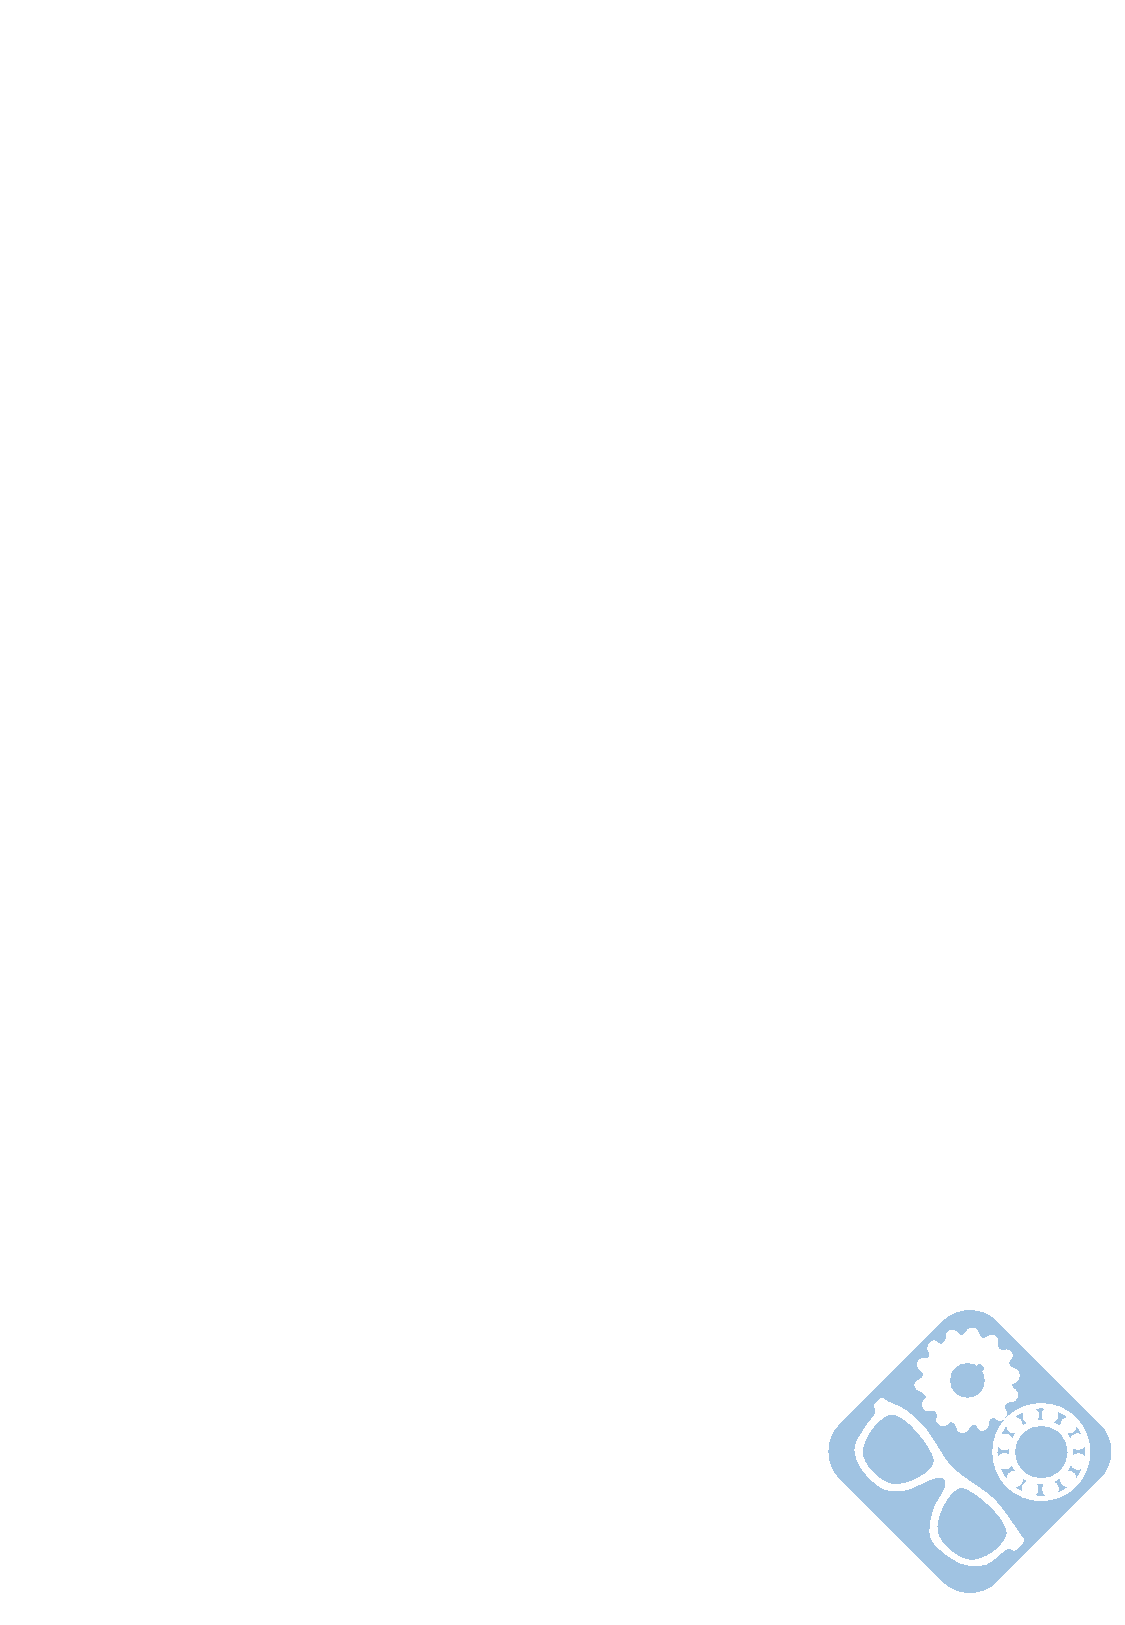
\includegraphics[width=\paperwidth,height=\paperheight,%
keepaspectratio]{../../img/fond4}%
\end{center}
\vfill
}}}

\begin{document}

\pagestyle{empty}

\AddToShipoutPicture*{\BackgroundPic}


\includegraphics[width=2cm]{../../img/logo}

\Huge{DS \num\ - \sujet}

\vspace{1cm}

\ifdef{\prive}{\begin{center}\colorbox{danger}{\Huge{Avec Correction}}\end{center}}{}

\begin{center}
\centering\huge{PTSI}
\end{center}

\vspace{2cm}


\begin{center}
\centering\Large{\jour}
\end{center}

\vspace{2cm}

\normalsize

\tableofcontents

\newpage

\AddToShipoutPicture{\BackgroundPicdeux}

\pagestyle{fancy}

\begin{center}
\Huge \sujet
\end{center}


\normalsize

\section{Présentation générale}

L'amélioration de la mobilité des personnes âgées ou rencontrant des troubles de la marche demeure un des enjeux majeurs de l'assistance à la personne.

Un dispositif d'assistance à la marche peut être prescrit lors de l'apparition de troubles de la locomotion. Parmi les nombreux dispositifs proposés, la canne et le déambulateur demeurent les plus utilisés ; l'utilisation de la canne étant privilégiée lors de troubles mineurs ou n'affectant qu'une des deux jambes.

Afin de contribuer à l'amélioration de l'assistance apportée par ces deux dispositifs conventionnels, la robotisation de ceux-ci a été entreprise. Ainsi, de nombreux déambulateurs robotisés ont été conçus afin d'offrir une assistance continue lors de la marche. En revanche, le développement des cannes robotisées s'est traduit par une différenciation marquée par rapport aux cannes conventionnelles (voir figure \ref{evo_cannes}). En effet, l'utilisation de bases mobiles stables sur lesquelles sont fixées des cannes, conduit à l'obtention de dispositif encombrant.

\begin{center}
\begin{tabular}{|c|c|c|}\hline
Canne & Canne à base  & Prototype de canne robotisée\\
conventionnelle & mobile stable  & étudié dans ce sujet\\
& composée de 3 roues & \\
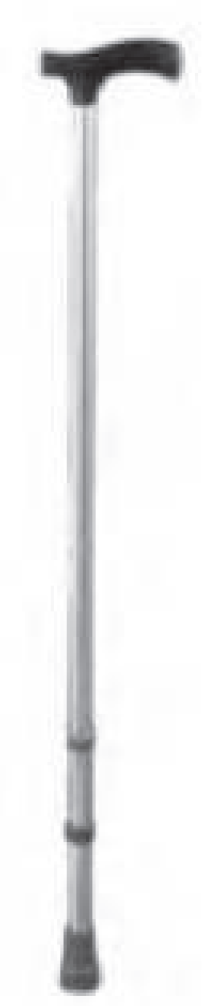
\includegraphics[width=1.5cm]{img/canneconv} & 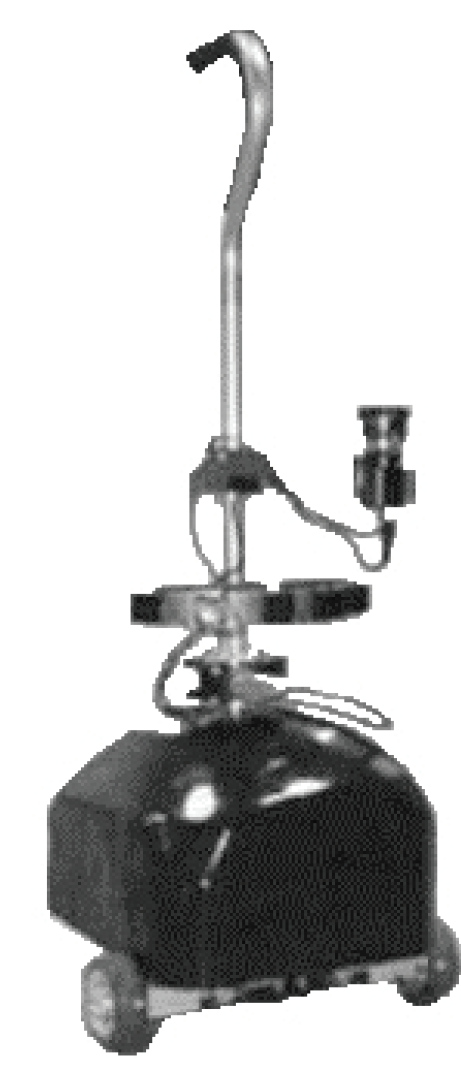
\includegraphics[width=3cm]{img/canne3roues}  & 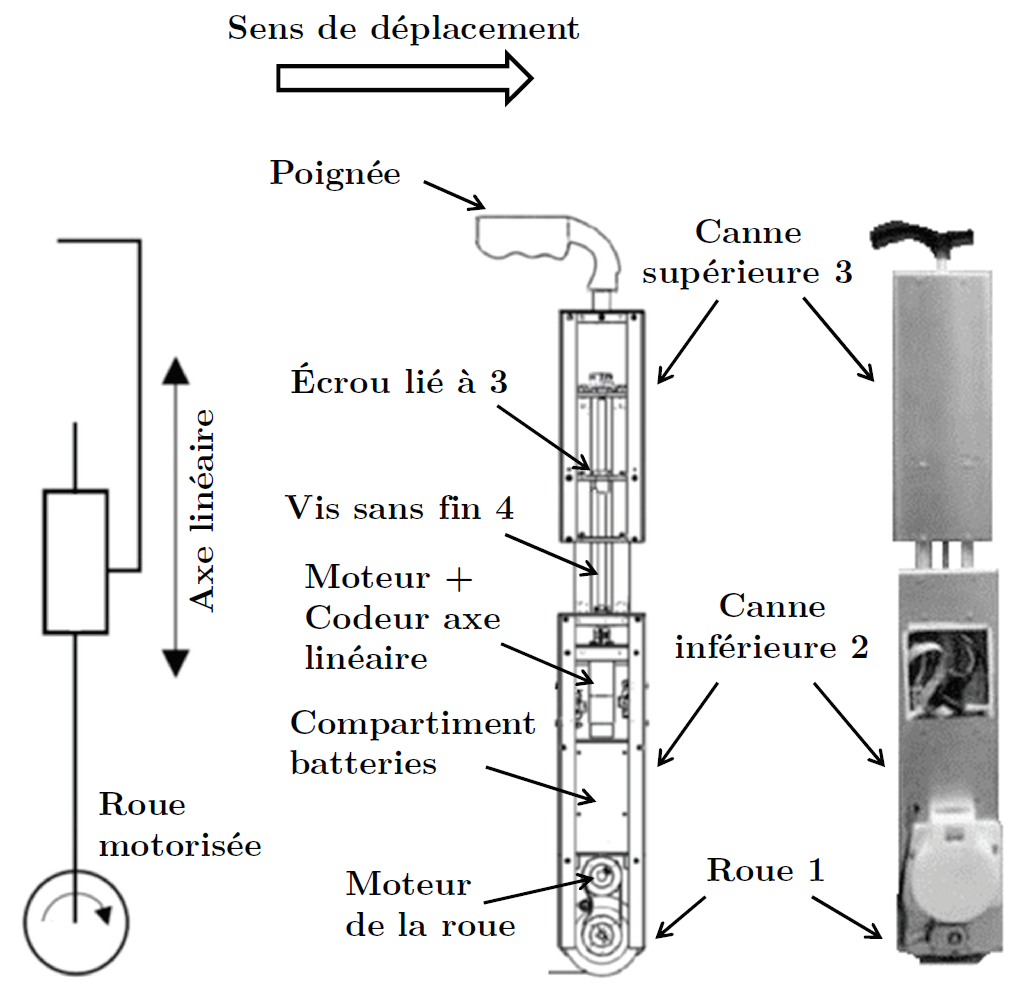
\includegraphics[width=9.5cm]{img/prescanne}\\\hline
\end{tabular}
\captionof{figure}{\label{evo_cannes}Évolution des dispositifs d'assistance à la locomotion de type canne et description du prototype de canne robotisée}
\end{center}

Pour plus de compacité et pour garder les attributs d'une canne conventionnelle, le prototype de canne étudié dans ce sujet est composé d'un axe télescopique et d'une roue à son extrémité, tous deux motorisés. Il conserve ainsi un encombrement réduit et permet de synchroniser les mouvements avec le cycle de la marche. La canne suit ainsi activement le mouvement de la jambe « invalide » durant la phase de balancement et offre un point d'appui stable pendant la phase d'appui.

L'extrait du cahier des charges donné dans le tableau ci-dessous reprend les principales exigences attendues par le comportement de la canne.

\begin{center}
\begin{tabular}{|c|c|c|}\hline
\textbf{Performance} & \textbf{Critère} & \textbf{Valeur}\\\hline
Précision & erreur statique & $\mu_s\leq 5\%$ \\\hline
Amortissement & 1er dépassement & $D_{1\%}\leq 5\%$ \\\hline
Rapidité & temps de réponse à 5\% & $tr_{5\%}\leq \SI{60}{ms}$ \\\hline
Stabilité & Marge de gain & $M_G \geq \SI{45}{db}$\\
 & Marge de phase  & $M_\varphi \geq \SI{35}{\degree}$\\\hline
\end{tabular}
\end{center}
\section{Analyse du cycle de la marche}

L'objectif de cette partie est d'étudier des cycles de marches saines et perturbées afin de mettre en évidence l'apport d'une canne d'assistance pour améliorer la marche. L'observation des jambes, effectuée dans le cadre d'un « cycle de marche », permet de distinguer pour chacune d'entre elle une phase d'appui et une phase de balancement (figure \ref{cymarche}). Ce cycle débute par un appui simple de la jambe droite et le début du balancement de la jambe gauche. Il s'achève lors du décollement du pied gauche du sol.

\begin{center}
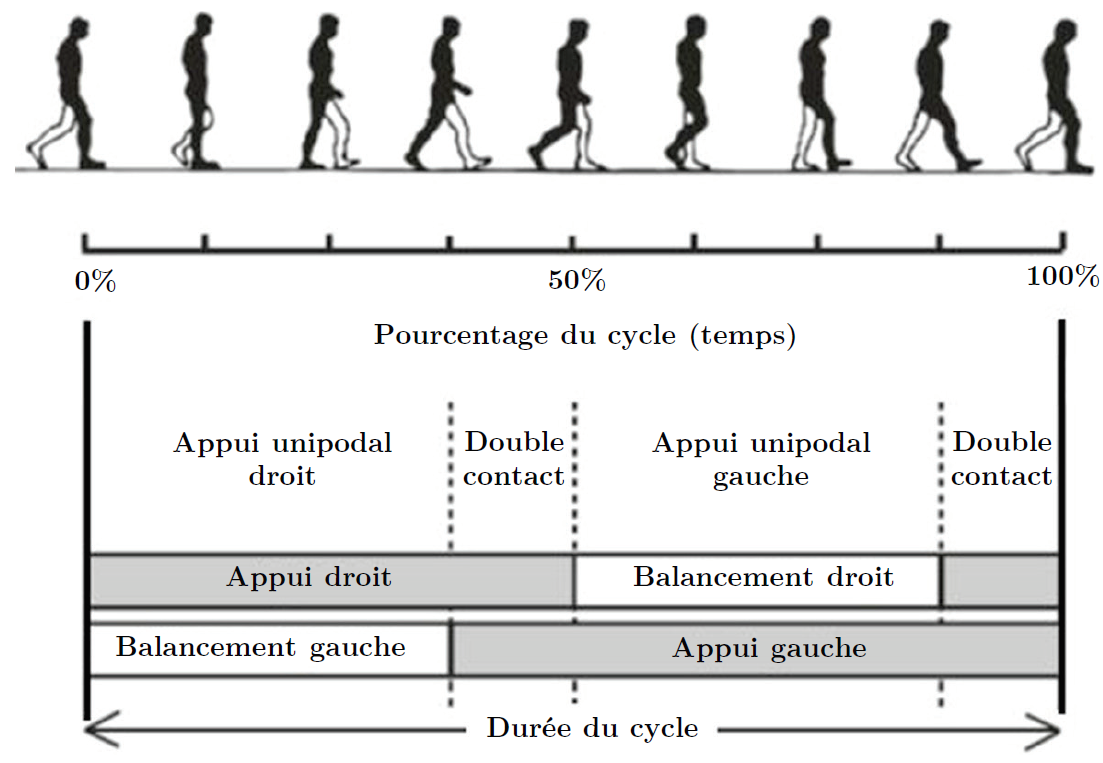
\includegraphics[width=10cm]{img/marche}
\captionof{figure}{\label{cymarche}Représentation du cycle de la marche adopté dans le cadre de notre étude} 
\end{center}

Les résultats obtenus pour les différentes conditions sont présentés sur les figures \ref{f4} à \ref{f7}. Ces courbes représentent l'évolution des efforts normaux (orthogonaux au sol) exercés par les jambes ou la canne sur le sol. Afin de faciliter l'observation des résultats, tous les résultats ont été normalisés, ceux relatifs à la jambe droite sont représentés en trait fort et ceux relatifs à la jambe gauche en trait fin. Les écarts-types associés aux résultats sont représentés en pointillés. Le trait continu représente la moyenne.

Pour ces figures, le cycle de la marche adopté durant l'étude débute par l'appui simple sur la jambe droite. La jambe gauche sera la jambe équipée des dispositifs contraignants dans le cadre de la marche perturbée et assistée d'une canne. Pour ce dernier cas, la canne est placée du côté de la jambe valide, c'est-à-dire du côté de la jambe droite.

\question{A partir de l'étude des figures \ref{f4} et \ref{f5}, comparer et commenter les évolutions des efforts normaux de chacune des jambes sur le sol et les durées de chacune des phases pour les différents cas : marche saine et marche perturbée.
}

\question{A partir de l'étude des figures \ref{f6} et \ref{f7}, préciser le rôle de la canne lors d'une marche assistée. %Préciser, en Newton, la valeur moyenne maximale des efforts exercés sur la canne.
}

\begin{center}
\begin{minipage}{0.48\linewidth}
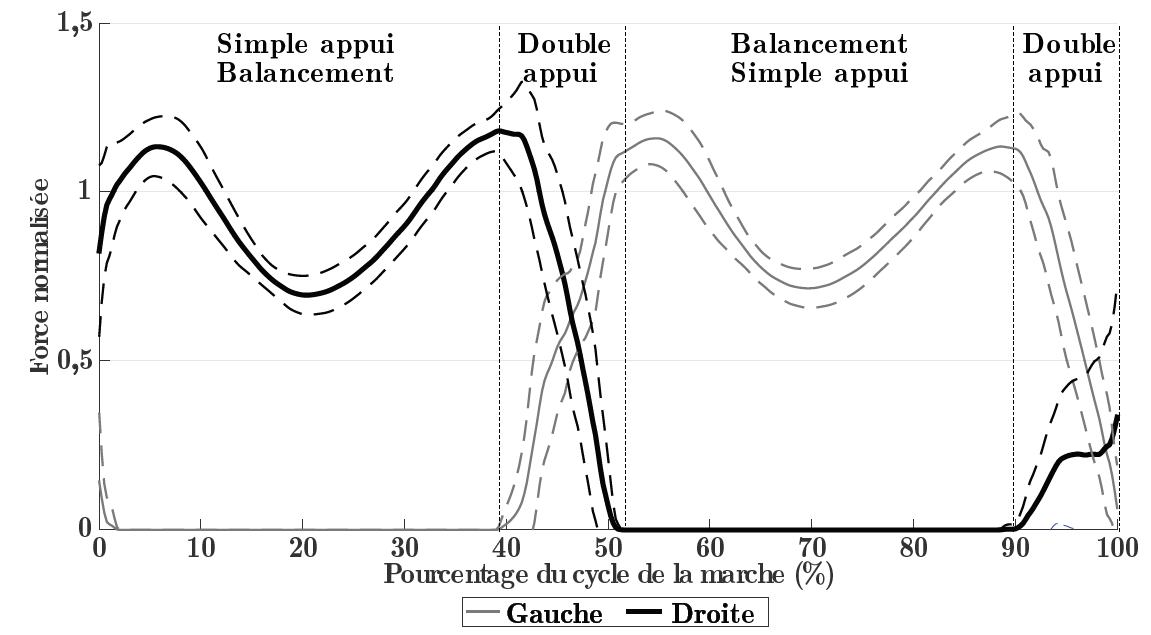
\includegraphics[width=\linewidth]{img/fig4}
\captionof{figure}{\label{f4}Efforts normaux générés par les jambes durant un cycle de marche normale à $V = \SI{0,45}{m/s}$}
\hspace{1cm}\\
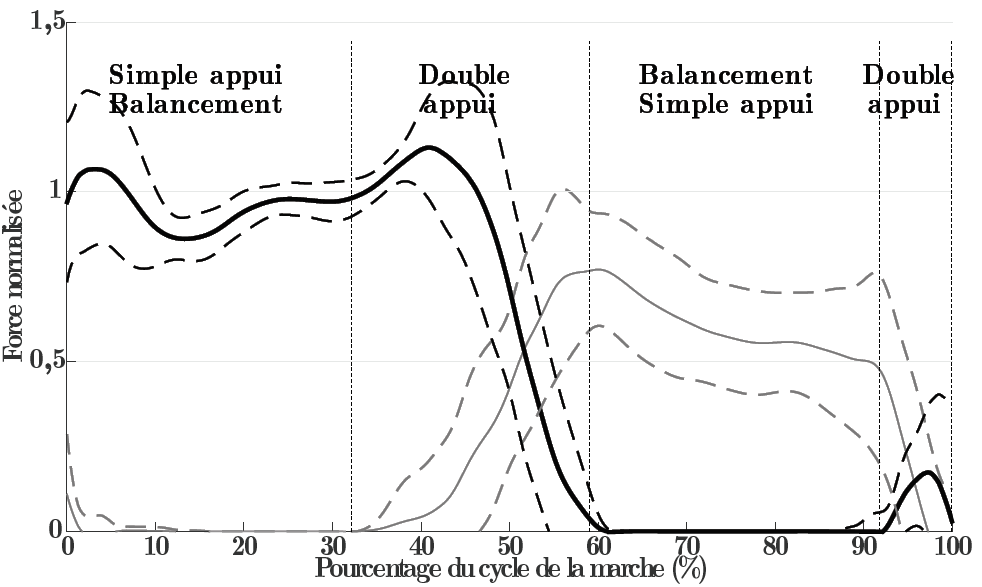
\includegraphics[width=\linewidth]{img/fig6}
\captionof{figure}{\label{f6}Efforts normaux générés par les jambes durant un cycle de marche assistée à allure moyenne, $V = \SI{0,22}{m/s}$} 
\end{minipage}\hfill \vrule \hfill
\begin{minipage}{0.48\linewidth}
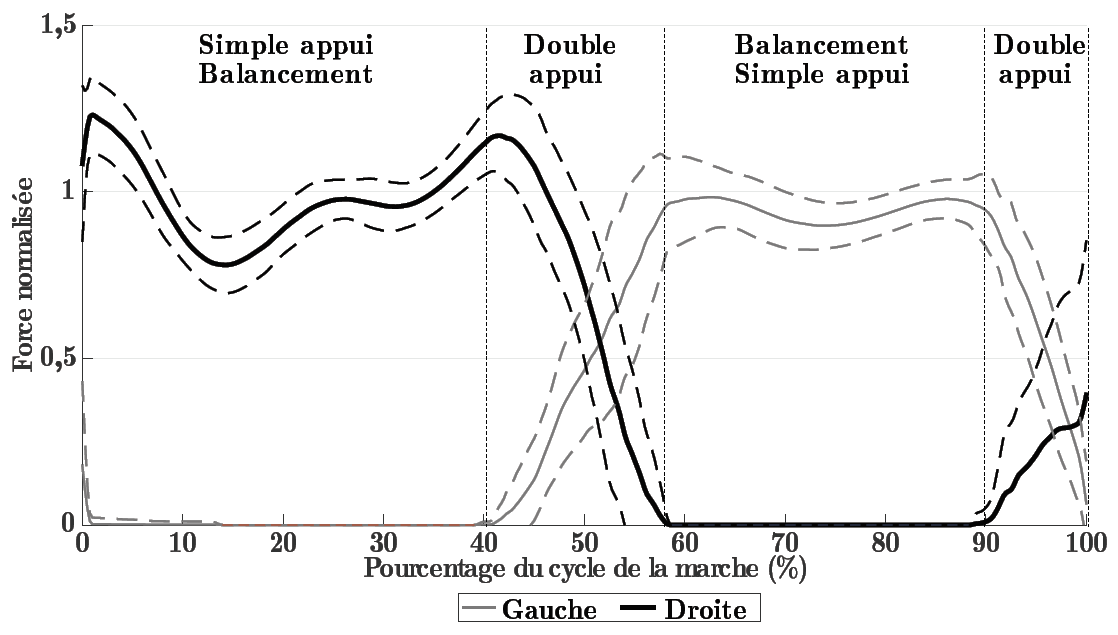
\includegraphics[width=\linewidth]{img/fig5}
\captionof{figure}{\label{f5}Efforts normaux générés par les jambes durant un cycle marche perturbée à allure moyenne, $V = \SI{0,22}{m/s}$}
\hspace{1cm}\\

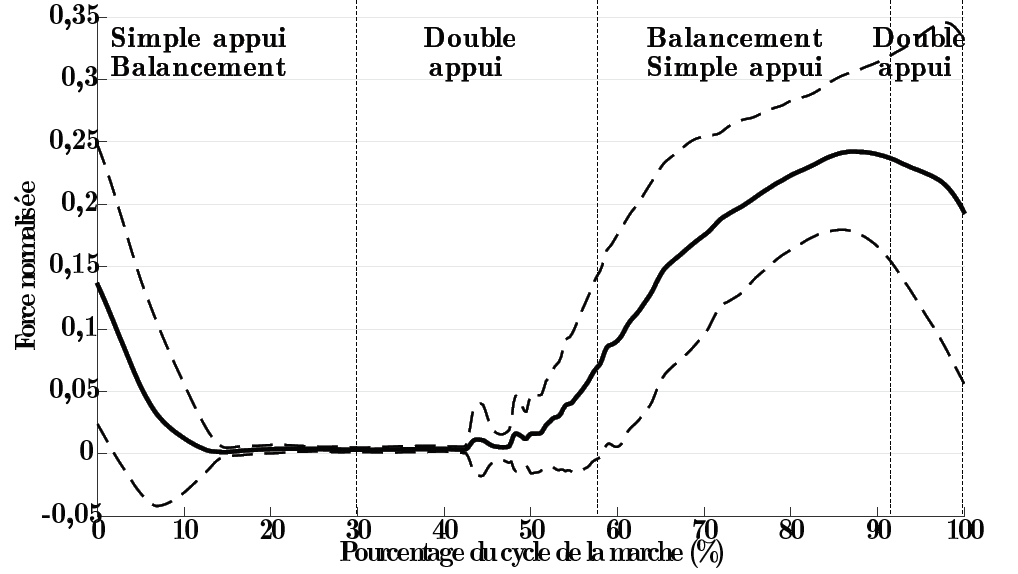
\includegraphics[width=\linewidth]{img/fig7}
\captionof{figure}{\label{f7}Efforts normaux générés par la canne durant un cycle de marche assistée à allure moyenne, $V = \SI{0,22}{m/s}$}
\end{minipage}
\end{center}

\section{Modélisation de la chaîne d'énergie de l'axe linéaire}

On considère que le moteur de l'axe linéraire (figure \ref{evo_cannes}) adopte le même comportement que celui d'un moteur à courant continu. Les équations de comportement sont rappelées ci-après :
\[u_m(t)=e(t)+ R i_m(t)+L\dfrac{\dd i_m(t)}{\dd t}, \qquad e(t)=K_e \omega_m(t) \quad \textrm{et} \quad c_m(t)=K_c i_m(t).\]

On notera $U_m(p)$ respectivement $I_m(p)$, $C_m(p)$ et $E(p)$ les transformées de Laplace des variables $u_m(t)$, la tension moteur, respectivement $i_m(t)$, le courant moteur, $c_m(t)$, le couple moteur et $e(t)$, la force contre-électromotrice.

Une étude énergétique a permis d'obtenir l'équation du mouvement \[J_{eq} \dfrac{\dd \omega_m(t)}{\dd t}+ f \omega_m(t)=c_m(t) - \dfrac{pas}{2\pi} F_p(t)\]

où $F_p(t)$ correspond à l'action mécanique (force) de la main de la personne sur la canne et où $R$, $L$, $K_e$, $K_c$, $J_{eq}$ et $f$ sont des constantes du moteur et $pas$ correspond au pas du système vis/écrou (pièces 3 et 4 sur la figure \ref{evo_cannes}).

\question{En supposant les conditions initiales nulles, déterminer, dans le domaine de Laplace, l'équation du mouvement précédente et compléter le schéma-blocs.}

\medskip
Soient $H_1(p)$ et $H_2(p)$ les fonctions de transfert telles que:  $\Omega_m(p)=H_1(p)\cdot U_m(p) + H_2(p)\cdot F_p(p)$.

\question{Déterminer les expressions littérales des formes canoniques des fonctions de transfert $H_1(p)$ et $H_2(p)$ en fonction des constantes du problème.
}

\medskip
Le dispositif vis/écrou (figure \ref{evo_cannes}), permettant la transformation de l'angle de rotation de la vis sans fin 4 (de $pas=\SI{3}{mm}$) en déplacement de l'écrou 3, est modélisé par un gain pur $K_{ve}=\dfrac{pas}{2\pi}=\SI{0.477}{mm.rad^{-1}}$.\\
Le comportement du codeur incrémental est modélisé par un gain pur $K_{codeur}=\SI{79.6}{inc.rad^{-1}}$. La sortie de ce bloc est de type numérique (en incréments) et son entrée est une position angulaire (en radians).
%\medskip
%}

%\Questionpb{Déterminer, à partir des données du diagramme de blocs internes, les expressions puis les valeurs numériques de $K_{ve}$ et $K_{codeur}$.}

%\Solution{}

%\Onlyproblem{
%\medskip
Afin d'asservir en déplacement le mouvement de la canne, un adaptateur de gain pur $K_{adapt}$ est placé en amont du comparateur de manière à convertir la consigne $X_c(p)$ en une grandeur en incréments directement comparable à la sortie $\theta_{mes}(p)$ du capteur. La valeur du gain pur $K_{adapt}$ est prise de manière à ce que l'écart $\varepsilon(p)$ soit nul lorsque $X_c(p) = X(p)$.
\medskip

\question{Donner l'expression, puis la valeur numérique et l'unité du gain pur $K_{adapt}$ permettant de satisfaire cette condition.}


\question{Compléter alors le schéma-bloc à retour unitaire du document réponse en fonction de $K_{codeur}$, $K_{ve}$, $C(p)$, $H_1(p)$ et $H_2(p)$. En déduire la fonction de transfert en boucle ouverte du système sans perturbation $H_{BO1}(p)$.
}

\section{Modèle comportemental}

Afin de proposer une modélisation simplifiée de la chaîne d'énergie de l'axe linéaire, une simulation du modèle précédent en boucle ouverte non perturbé notée $H_{BO1}(p)$ a été réalisée. On considère que $H_{BO1}(p)$ est de la forme $H_{BO1}(p)=\dfrac{K_{BO}}{p(1+T_1p)(1+T_2p)}$ avec $T_1 < T_2$.
Le document réponse présente la réponse fréquentielle du système en boucle ouverte à l'aide du diagramme de Bode (courbe de gain $G_{BO}(\omega)$ et courbe de phase $\varphi_{BO}(\omega)$).
\medskip

\question{Représenter le tracé asymptotique de $H_{BO1}(p)$ sur le diagramme de Bode et en déduire les valeurs de $T_1$, $T_2$ et $K_{BO}$. On rappelle que $10^{3/2}=\sqrt{1000}\approx32$.}


%\Onlyproblem{
%\medskip
%Lors d'une marche saine à allure rapide la cadence moyenne est de 113 pas par minute.
%\medskip}
%
%\Questionpb{\label{freq} Déterminer la fréquence moyenne en Hz de la marche saine à allure rapide.}
%
%\Solution{$F=\dfrac{113}{60}\approx \SI{1,83}{Hz}$}

\medskip
On considère que la fréquence maximale de déplacement de l'axe linéaire de la canne (liée au mouvement de la marche) est fixée à $F_{max} =\SI{4}{Hz}$. Une première approximation du comportement du système en boucle ouverte est proposée par une fonction de transfert $H_{BO}(p)$ de la forme $H_{BO}(p) = \dfrac{K_{BO}}{p}$ avec $K_{BO} = 1/30$ pour des fréquences inférieures à $F_{max}$.
\medskip

\question{Justifier la validité de cette modélisation approchée à l'aide de la réponse fréquentielle du système en boucle ouverte (voir DR \textbf{Q\ref{7}}).}

\section{Correction proportionnelle}

Pour la suite, on modélise le comportement du système en boucle ouverte par $H_{BO}(p) = \dfrac{K_{BO}}{p}$ avec $K_{BO} = 1/30$. On considère un correcteur à action proportionnelle tel que $C(p)= K_{corr}$.

Le schéma-bloc du système non perturbé correspond alors à celui de la figure \ref{sb_corr_prop}.

%\begin{figure}[htbp]\centering
%	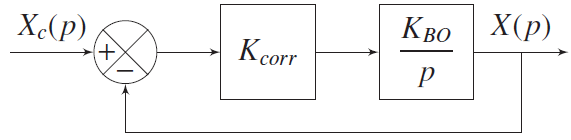
\includegraphics[width=7cm]{sb_corr_prop}

%\end{figure}
\begin{center}
\begin{tikzpicture}
			\sbEntree{E1}
			\sbComp{C1}{E1}
				\sbRelier[$X_c(p)$]{E1}{C1}
			\sbBloc{B1}{$K_{corr}$}{C1}
				\sbRelier{C1}{B1}
			\sbBloc{B2}{$H_{BO}(p)=\dfrac{K_{BO}}{p}$}{B1}
				\sbRelier{B1}{B2}
			\sbSortie[3]{S1}{B2}
				\sbRelier[$X(p)$]{B2}{S1}
			\sbRenvoi{B2-S1}{C1}{}	
\end{tikzpicture}
\captionof{figure}{Schéma-bloc simplifié du système non perturbé avec $C(p)=K_{corr}$\label{sb_corr_prop}}
\end{center}

\question{Déterminer l'expression littérale de la forme canonique de $H_{BF}(p) = \dfrac{X(p)}{Xc(p)}$, fonction de transfert en boucle fermée de la modélisation de la figure  \ref{sb_corr_prop}.}

\question{Déterminer les paramètres caractéristiques de $H_{BF}(p)$ et en déduire les performances de cette modélisation pour $C(p)= K_{corr} = 1$. Conclure vis-à vis des exigences d'asservissement de l'axe linéaire.}

\medskip
On se propose de modifier la valeur de $K_{corr}$ de manière à vérifier l'exigence de rapidité de l'asservissement.
\medskip

\question{Quelle est l'influence de la modification du gain $K_{corr}$ sur les diagrammes de Bode de la fonction de transfert en boucle ouverte.}

\question{Déterminer la valeur numérique à donner à $K_{corr}$ pour assurer le temps de réponse à 5\% lié à l'exigence de rapidité de de l'asservissement de l'axe linéaire.}

\medskip
La figure \ref{sanscor} donne l'évolution de la réponse temporelle $x(t)$ du système réel non perturbé à un échelon en déplacement de valeur finale $x_0 = \SI{10}{mm}$, pour une correction proportionnelle $K_{corr} = \SI{1500}{}$.

\begin{center}
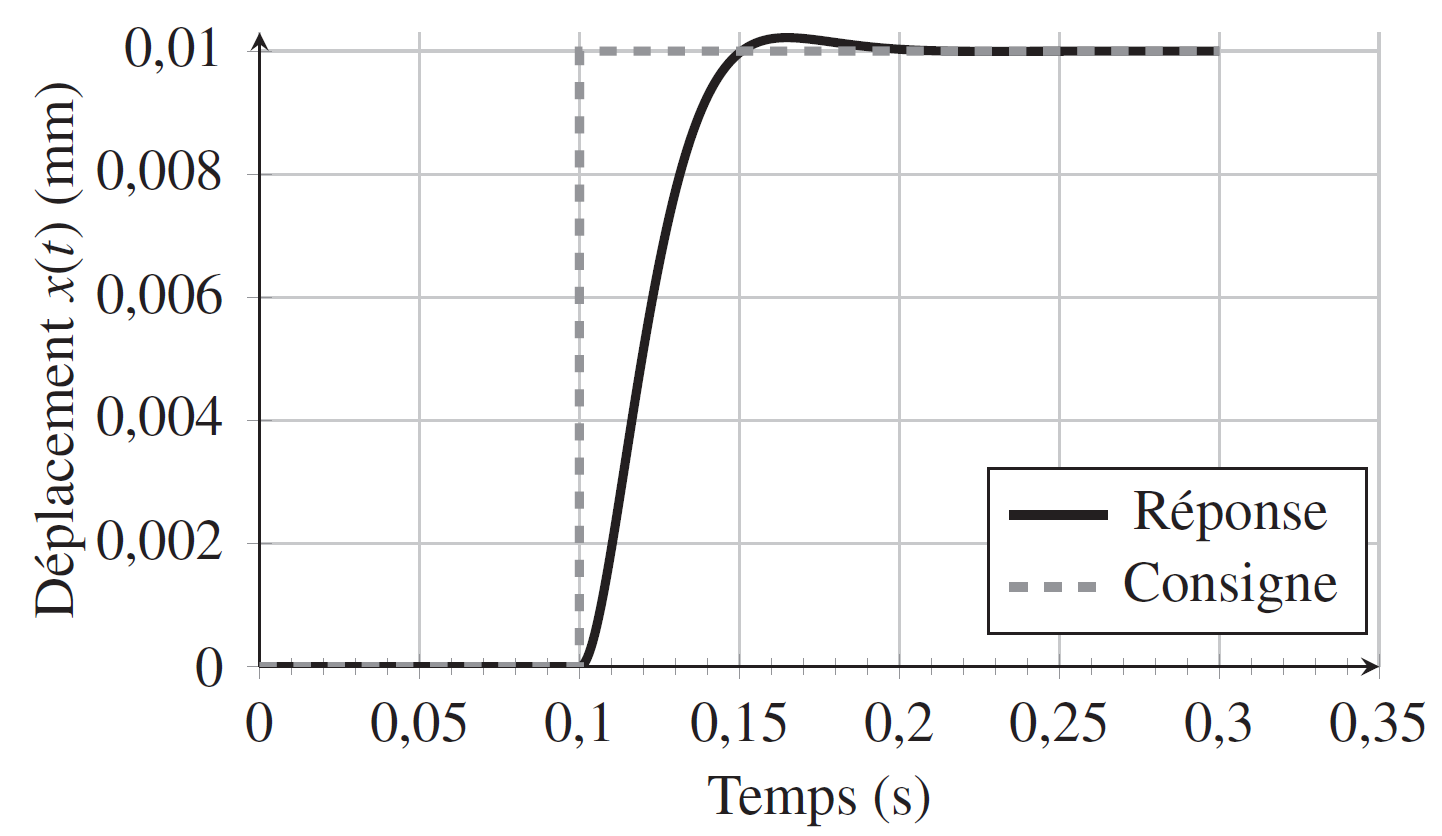
\includegraphics[width=8cm]{img/repind}
\captionof{figure}{\label{sanscor}Évolution de la réponse temporelle $x(t)$ du système réel non perturbé à un échelon de valeur $x_0 = \SI{10}{mm}$, pour $K_{corr} = \SI{1500}{}$}
\end{center}

\question{L'évolution de la réponse du système est-elle cohérente avec le comportement du modèle retenu ? Justifier. Quelle modification faudrait-il apporter au modèle approché pour retrouver cette forme de réponse temporelle ?}

Pour la suite, on modélise la fonction de transfert en boucle ouverte du système par \[H_{BO}(p) = \dfrac{1}{p}\cdot\dfrac{K_{BO}}{1+\tau_{BO}p} \textrm{ avec } K_{BO} =\dfrac{1}{30} \SI{}{s^{-1}} \textrm{ et } \tau_{BO} = \SI{9}{ms}.\]

\question{Donner la forme canonique de la nouvelle fonction de transfert $H_{BF}(p) = \dfrac{X(p)}{Xc(p)}$ toujours pour une correction proportionnelle de gain $K_{corr}$ et identifier ses paramètres caractéristiques.}

\question{Quelle valeur maximale de $K_{corr}$, notée $K_{corr}^{MAX}$ , permet de vérifier les critères de précision et de dépassement de l'asservissement de l'axe linéaire ?}

\question{Déterminer la valeur du temps de réponse à 5 \% de ce modèle pour $K_{corr}=K_{corr}^{MAX}$ à partir de l'abaque du temps de réponse réduit (figure \ref{abaque}).
}



\begin{figure}[htbp]\centering
	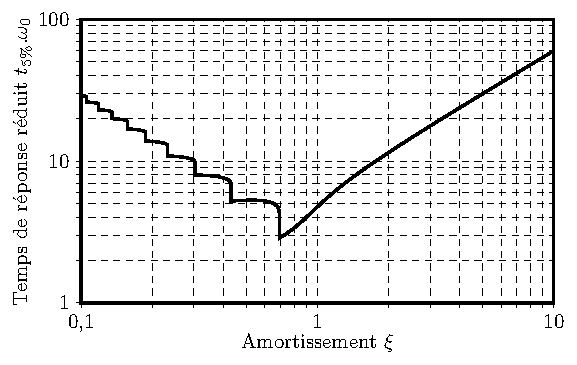
\includegraphics[width=9cm]{img/figure5}
	\captionof{figure}{Abaque des temps de réponse réduit\label{abaque}}
\end{figure}

La figure \ref{repcor} donne les évolutions des réponses temporelles $x(t)$ du système réel avec prise en compte de la perturbation ($F_p$ constante et égale à \SI{175}{N}) à un échelon en déplacement de valeur finale $x_0 = \SI{10}{mm}$, pour une correction proportionnelle $K_{corr} = \SI{1500}{}$ et pour $K_{corr}=K_{corr}^{MAX}$.

\noindent
\begin{figure}[!h]\centering
	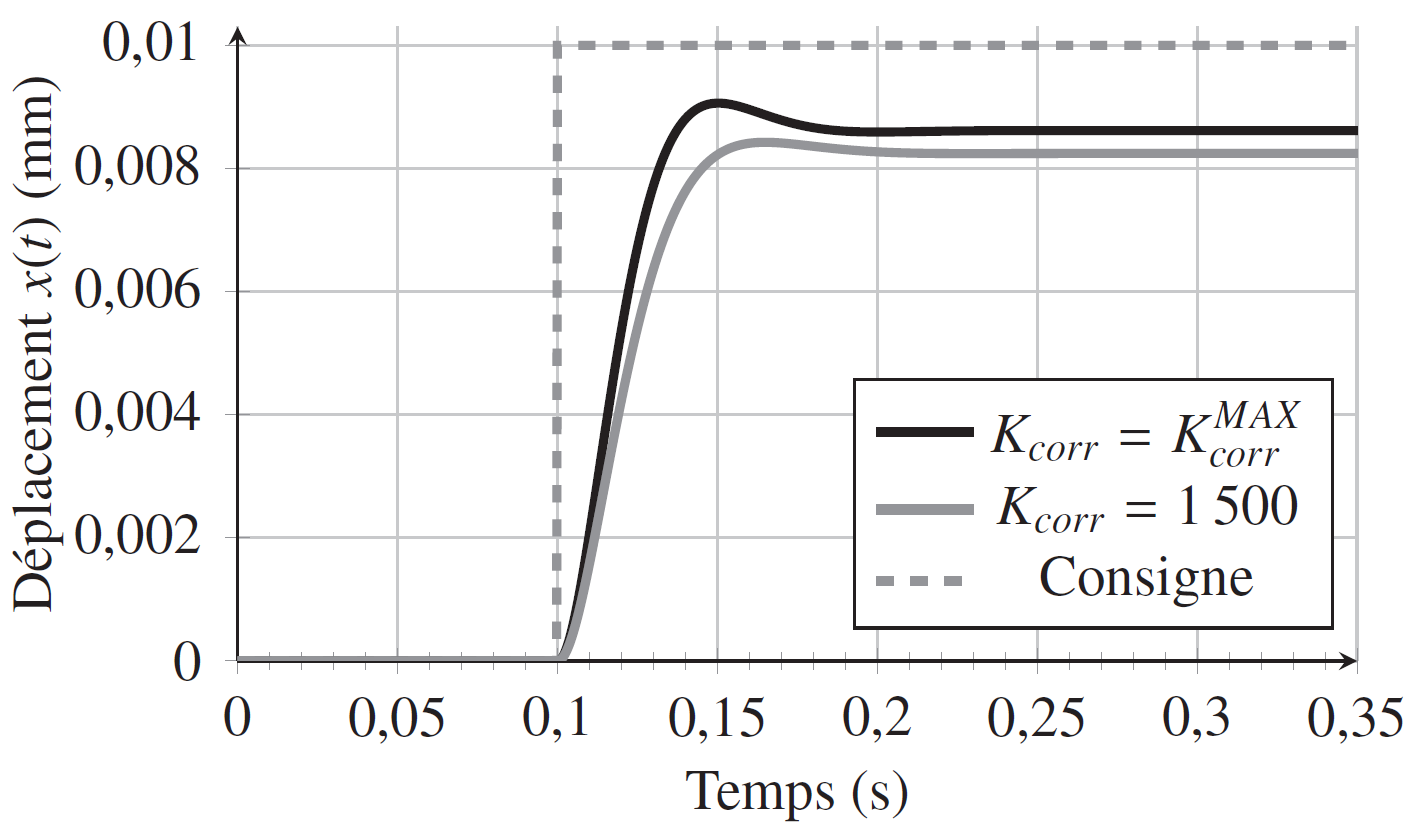
\includegraphics[width=9cm]{img/repindcor}
	\captionof{figure}{\label{repcor}Réponses indicielles $x(t)$ du système perturbé ($x_c = \SI{10}{mm}$), pour différents gains de correction proportionnelle $K_{corr}$}
\end{figure}

\medskip

\question{Conclure sur les capacités de la correction à action proportionnelle pure vis-à-vis des performances à atteindre.}

\section{Correction avec action proportionnelle et intégrale généralisée}

Le correcteur finalement retenu est un correcteur avec action proportionnelle et intégrale généralisée. La fonction de transfert $C(p)$ prend alors la forme suivante :

\begin{center}
$C(p)=K_{corr} \cdot \dfrac{1+T_d p}{p}$ avec $K_{corr} \gg 1$ et $T_d<\SI{1}{s}$.
\end{center}

\question{Montrer que $FTBO(p)=\dfrac{K_{BO}\cdot K_{corr}\cdot(1+T_d p)}{p^2\cdot (1+\tau_{BO}\cdot p)}$}

\medskip

\question{Montrer qu'il existe un $\omega_1$ et un $\omega_2$, tel que:
\begin{itemize}
 \item si $\omega<\omega_1$, alors $(1+T_d j \omega)\approx 1$ et $(1+\tau_{BO} j \omega)\approx 1$,
 \item si $\omega_1<\omega<\omega_2$, alors $(1+T_d j \omega)\approx T_d j \omega$ et $(1+\tau_{BO} j.\omega)\approx 1$
 \item si $\omega_2<\omega$, alors $(1+T_d j \omega)\approx T_d j \omega$ et $(1+\tau_{BO} j\omega)\approx \tau_{BO} j.\omega$,
\end{itemize}

Déterminer $\omega_1$ et un $\omega_2$.
} 

\medskip

\question{En utilisant les approximations précédentes, déterminer l'expression simplifiée de $FTBO(p)$ dans les 3 cas précédents et compléter le tableau du document réponse.} 

La figure \ref{bode} représente les diagrammes de Bode du système en boucle ouverte avec correcteur PI Généralisé pour $K_{corr} = \SI{1000}{}$ et $T_d=\SI{0.2}{s}$.

\begin{figure}[!h]\centering
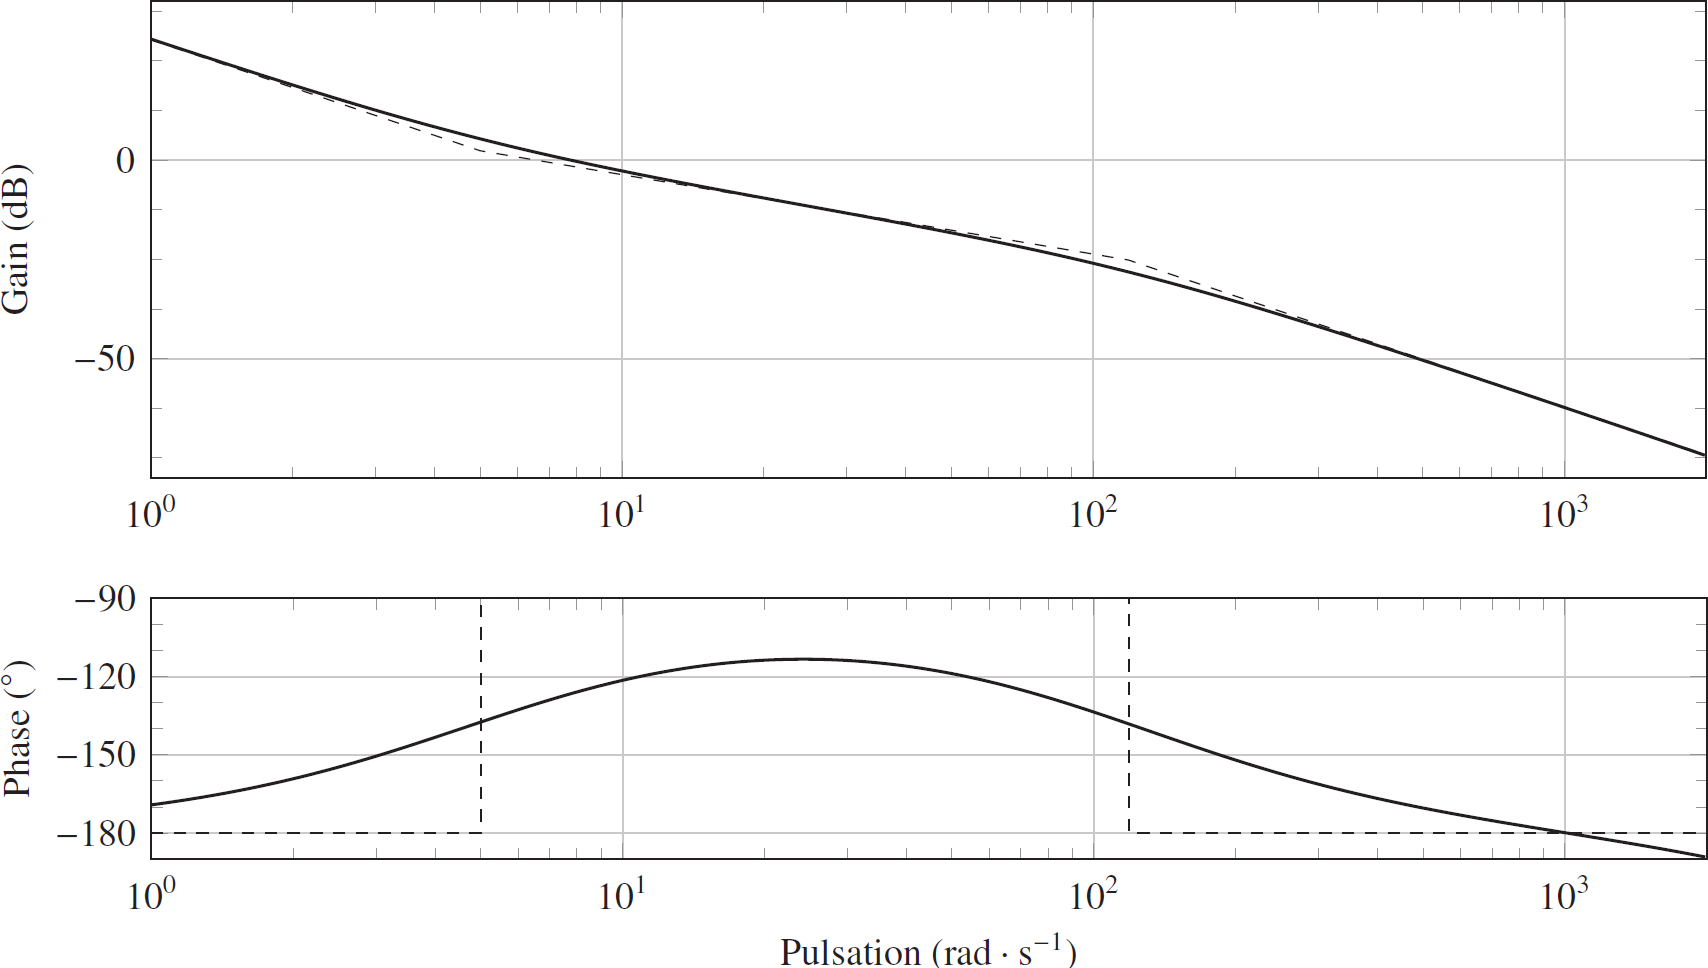
\includegraphics[width=.74\linewidth]{img/bodePI}
\captionof{figure}{\label{bode}Diagrammes de Bode du système en boucle ouverte avec correcteur PI Généralisé avec $K_{corr} = \SI{1000}{}$ et $T_d=\SI{0.2}{s}$}
\end{figure}

%On définit la marge de phase $M_\varphi$ comme la différence entre \SI{-180}{\degree} et la phase réelle pour la pulsation $\omega_1$ telle que le gain en décibel soit égal à \SI{0}{dB} pour cette pulsation, c'est-à-dire
%\begin{center}
%\fbox{$M_\varphi=\varphi(\omega_1)-(-180)=180+\varphi(\omega_1)$ avec $\omega_1$ telle que $G_{dB}(\omega_1)=0dB$}.
%\end{center}
%On définit la marge de gain $M_{G}$ comme la différence entre le gain réel pour la pulsation $\omega_2$ telle que la phase soit égale à \SI{-180}{degrés} pour cette pulsation et la gain nul, c'est-à-dire 
%\begin{center}
%\fbox{$M_{G}=G_{db}(\omega_2)-0 db$}.
%\end{center}


\question{Justifier le comportement asymptotique des diagrammes de Bode à partir des résultats précédents.}

%\Questionpb{\label{marges}Représenter sur le \DR{bode} les marges de gain $M_G$ et de phase $M_\varphi$ du système corrigé. Les performances de stabilité sont-elles vérifiées ?.}
%
%\Solution{On mesure la marge de phase à environ $M_\varphi\approx \SI{50}{\degree}$ et la marge de gain à $M_G\approx \SI{60}{db}$. ces deux marges sont supérieures aux valeurs minimales imposées par le cahier des charges. Les performances de stabilité sont vérifiées.}

\medskip
Avec cette correction, le système est précis mais les valeurs de marge de gain\footnote{Marge de gain $M_{G}$ : différence entre le gain réel pour la pulsation particulière $\omega$ telle que pour cette pulsation la phase soit égale à \SI{-180}{\degree} et le gain nul.} et marge de phase\footnote{Marge de phase $M_\varphi$ : différence entre \SI{-180}{\degree} et la phase réelle pour la pulsation $\omega_1$ telle que pour cette pulsation le gain en décibel soit égal à \SI{0}{dB}.} sont telles que le système n'est pas assez rapide. La valeur du gain $K_{corr}$ a donc été ajustée pour se rapprocher des valeurs limites de marges de gain et de phase autorisées.
\medskip

%\Questionpb{\label{kcorr}Quelle est l'influence de la modification du gain $K_{corr}$ sur les diagrammes de Bode de la fonction de transfert en boucle ouverte. En déduire la valeur maximale à donner au gain $K_{corr}$ pour respecter les performances en stabilité de l'asservissement de l'axe linéaire tout en augmentant au maximum la bande passante du système.}
%
%\Solution{L'augmentation du gain $K_{corr}$ entraine une translation de la courbe de gain uniquement selon l'axe des ordonnées. On voit qu'il est possible de translater la courbe de gain vers le haut de \SI{15}{db} (augmentation de la banque passante) pour atteindre la marge de gain minimale fixée par le cahier des charges (\SI{45}{db}). Comme le gain $K_{corr}$ valait initialement 1000, le nouveau gain $K_{corr}$ vaut $20\log{K_{corr}}=20\log{1000}+15$ soit $K_{corr}\approx 5623$.}

\medskip
Les figures \ref{repPI}a et \ref{repPI}b, donnent les évolutions temporelles de la position $x(t)$ du système simulé, perturbé et corrigé du déplacement $x(t)$ (en mm) et de l'intensité simulée (en Ampères) circulant au sein du moteur pour une consigne de déplacement $x_c(t)=x_0 u(t)$ d'amplitude $x_0 = \SI{10}{mm}$.

\begin{figure}[!h]\centering
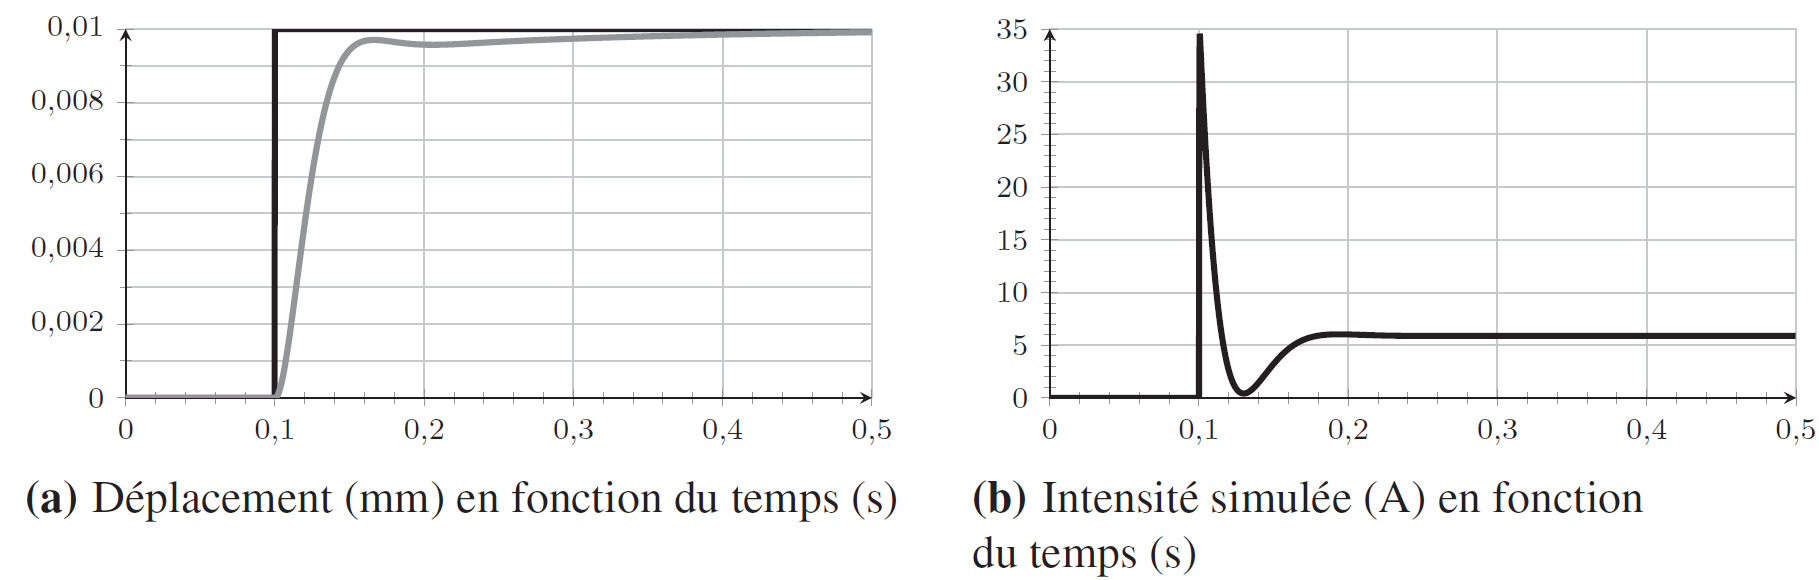
\includegraphics[width=\linewidth]{img/repindPI}
\captionof{figure}{\label{repPI}Évolutions temporelles du déplacement $x(t)$ et de l'inténsité $i(t)$ du système simulé, perturbé et corrigé, soumis à un échelon d'amplitude $x_0 = \SI{10}{mm}$} 
\end{figure}

Le variateur du moteur permet de protéger les éléments électroniques des surintensités qui pourraient apparaître lors de la commande. Afin de prendre en compte cette protection, on décide d'ajouter un bloc saturation de valeur $\pm \SI{20}{A}$ dans le modèle causal (voir question \ref{3}).


\question{Préciser, juste avant ou juste après quel bloc du \textbf{schéma-blocs de la question \ref{3}}, il faudra placer ce bloc saturation. %Justifier.
}

\medskip
Les figures \ref{repsat}a et \ref{repsat}b donnent respectivement la réponse temporelle du déplacement (en mm) à un échelon de consigne $x_0 = \SI{10}{mm}$ et l'évolution de l'intensité simulée (en Ampère) circulant au sein du moteur pour le système corrigé avec perturbation et ajout du bloc saturation $\pm \SI{20}{A}$.

\begin{figure}[!h]\centering
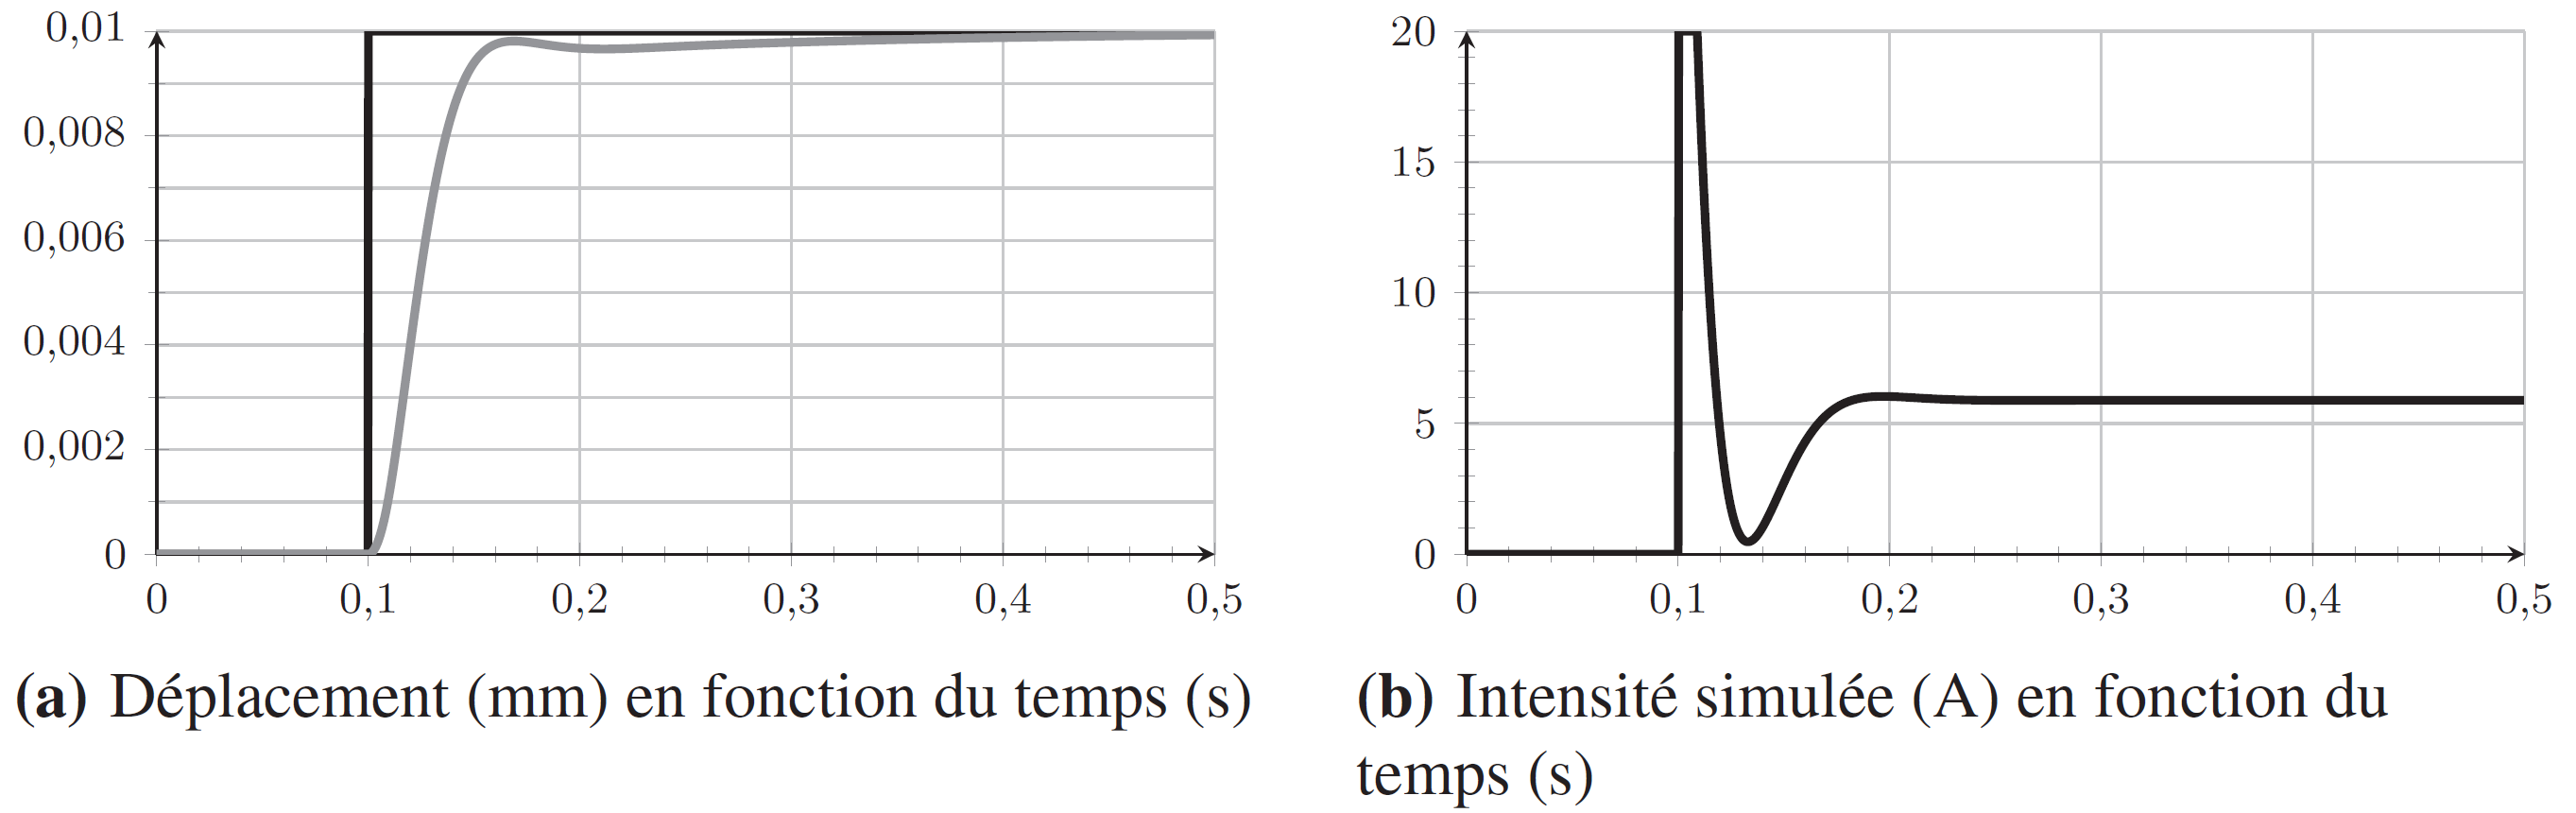
\includegraphics[width=\linewidth]{img/repindPIsat}
\captionof{figure}{\label{repsat}Évolutions temporelles du déplacement $x(t)$ et de l'intensité $i(t)$ du système simulé, perturbé et corrigé, soumis à un échelon d'amplitude $x_0 = \SI{10}{mm}$ avec bloc de saturation $\pm \SI{20}{A}$} 
\end{figure}

\question{Quel est l'effet de l'ajout du bloc saturation en intensité sur les performances du système ? Conclure vis-à-vis des exigences du cahier des charges.}

\section{Étude de l'exigence 3.1.6 « Commande des axes asservis »}
Cette partie a pour objectif d'analyser le mode de distinction des différentes phases de fonctionnement de la canne robotisée.

Lors de la marche avec une canne conventionnelle, il est possible de constater une synchronisation du mouvement de la canne conventionnelle avec celui de la jambe qu'elle assiste. Ainsi, une forte corrélation est observée entre l'angle de la canne et celui de la hanche de la jambe invalide.

\begin{figure}[!h]\centering
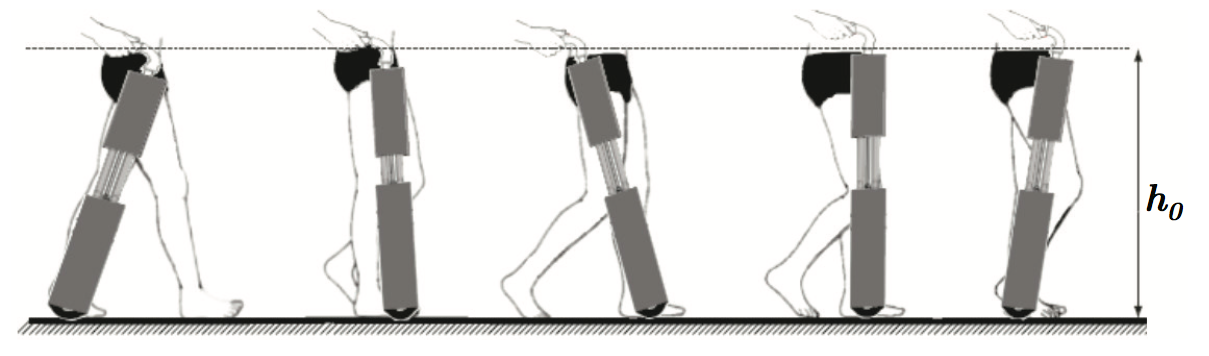
\includegraphics[width=0.7\linewidth]{img/fig_11_sujet_init}
\caption{\label{repsat}Synchronisation souhaitée du prototype de canne robotisée avec la marche}
\end{figure}

Selon la figure \ref{repsat}, le mode de commande suivant a été retenu pour contrôler le mouvement du proto-type de canne robotisée.
\begin{itemize}
 \item Lors de la phase de balancement de la jambe invalide, l'angle de la canne active par rapport à la verticale est asservi sur l'angle de la hanche de la jambe invalide. Cette tâche est accomplie
en gardant la hauteur de la poignée h 0 constante afin de ne pas perturber la position de la main
de l'utilisateur,
 \item Lors de la phase d'appui de la jambe invalide, la roue est asservie à une vitesse nulle afin d'offrir un point d'appui immobile pour le patient. La longueur de l'axe télescopique est asservie pour garder la hauteur de la poignée h 0 constante de la canne.
\end{itemize}

Il est donc nécessaire de maintenir la hauteur de poignée h 0 constante pour les deux phases. Ceci
impose une relation entre l'inclinaison de la canne et sa longueur.

\begin{figure}[!h]\centering
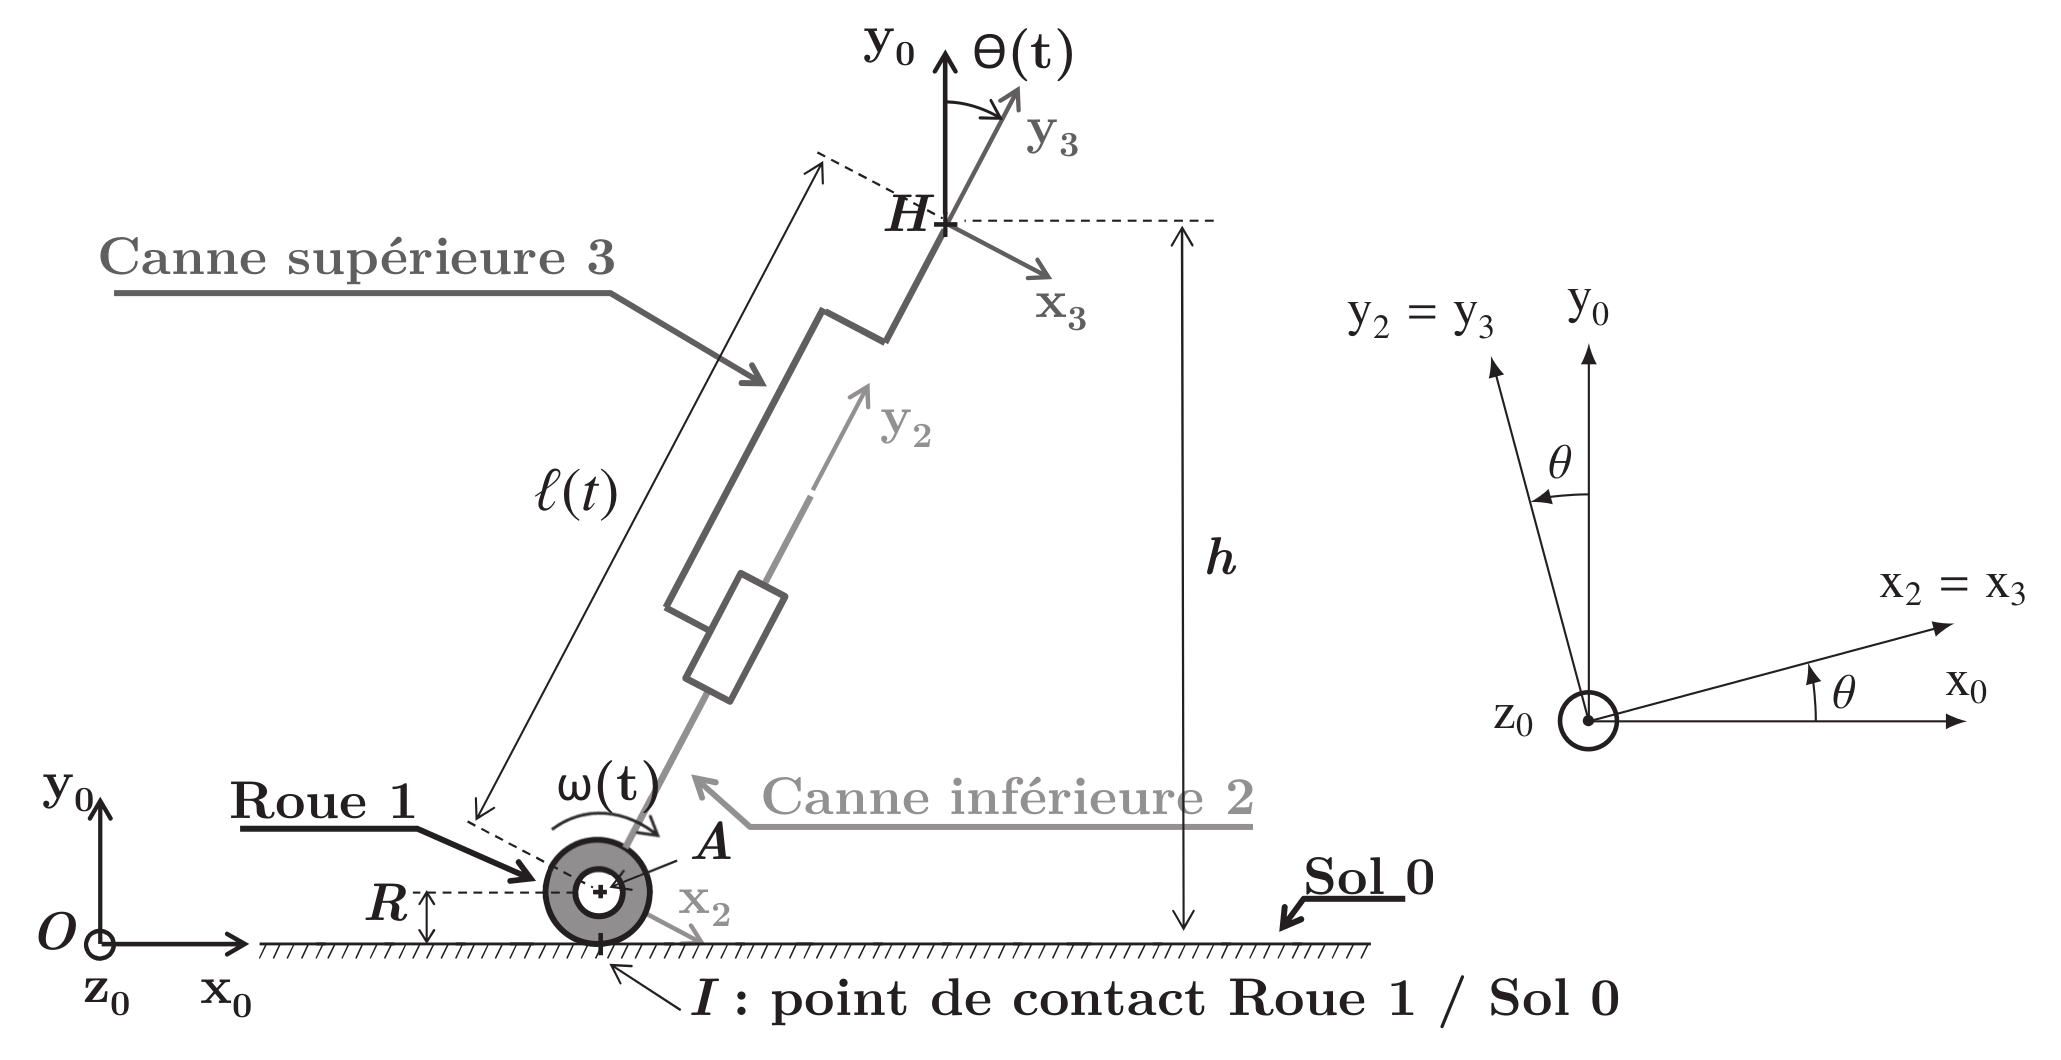
\includegraphics[width=0.9\linewidth]{img/fermeture_geo}
\caption{\label{ferm_geo}Modélisation cinématique et paramétrage du prototype de canne robotisée}
\end{figure}

La figure \ref{ferm_geo} présente le modèle cinématique et les notations retenues pour le paramétrage du prototype de canne. Sur cette figure, $l(t)$ représente la longueur AH, $\theta(t)$ correspond à l'angle d'inclinaison de la canne avec la verticale et R est le rayon de la roue. On note de plus $h$ la hauteur de poignée de la canne par rapport au sol.

\question{Établir la relation entre $l(t)$, $\theta(t)$ et $R$ pour assurer une hauteur constante $h=h_0$.}

\begin{figure}[!h]\centering
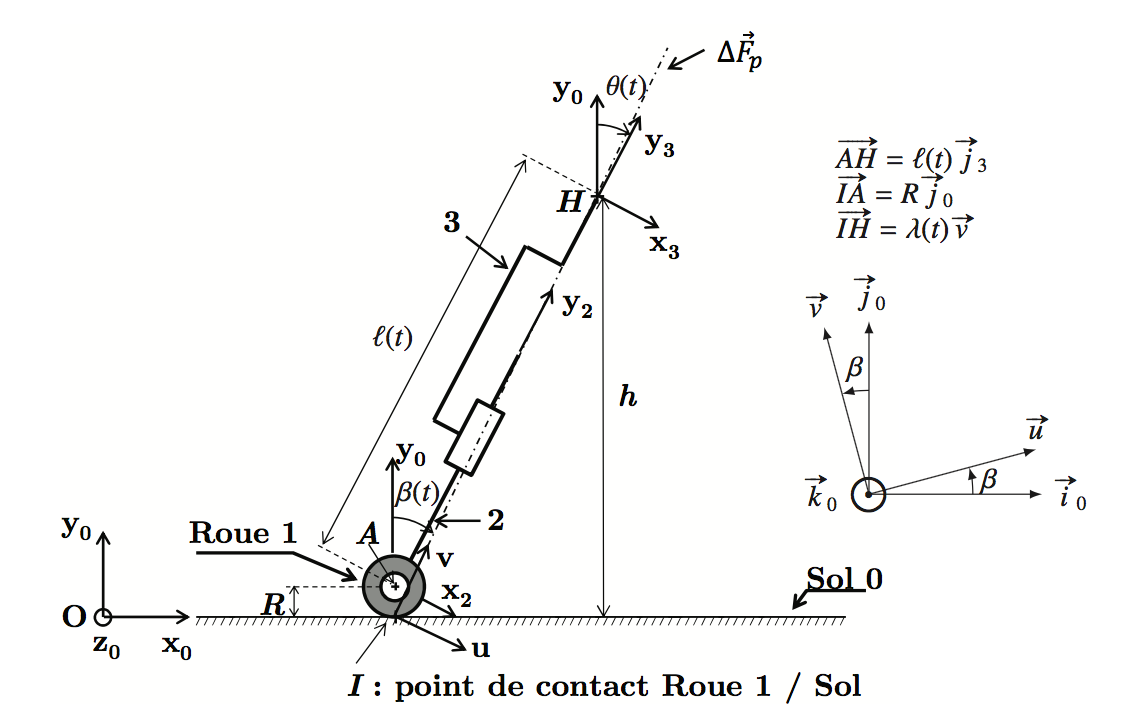
\includegraphics[width=0.9\linewidth]{img/fermeture_geo_2}
\caption{\label{ferm_geo2}Modélisation et paramétrage du prototype de canne robotisée}
\end{figure}

Dans la suite, on se propose de déterminer par une étude géométrique la relation entre $\beta(t)$, les données dimensionnelles $R$ et $h$ et l'angle $\theta(t)$. Pour cela, on introduit la base ($\vec{u},\vec{v},\vec{k_0})$ et on note $\lambda(t)$ la distance IH, telle que $\overrightarrow{IH} = \lambda(t).\vec{v}$.

\question{En développant une fermeture vectorielle en projection dans la base $B_0$, donner deux équations algébriques. En déduire la relation entre $\beta(t)$, $\theta(t)$, $l(t)$ et $R$.}

\question{Montrer à partir de ce résultat et de celui de la question que:

\begin{center}
$tan(\beta(t))=\frac{h-R}{h}.tan(\theta(t))$
\end{center}}

\section{Dessin}

\question{Compléter les vues manquantes sur le document réponse. Suivre l'exemple du premier dessin complété.}

\begin{center}
\huge{-- FIN --}
\end{center}

\newpage

\cleardoublepage

%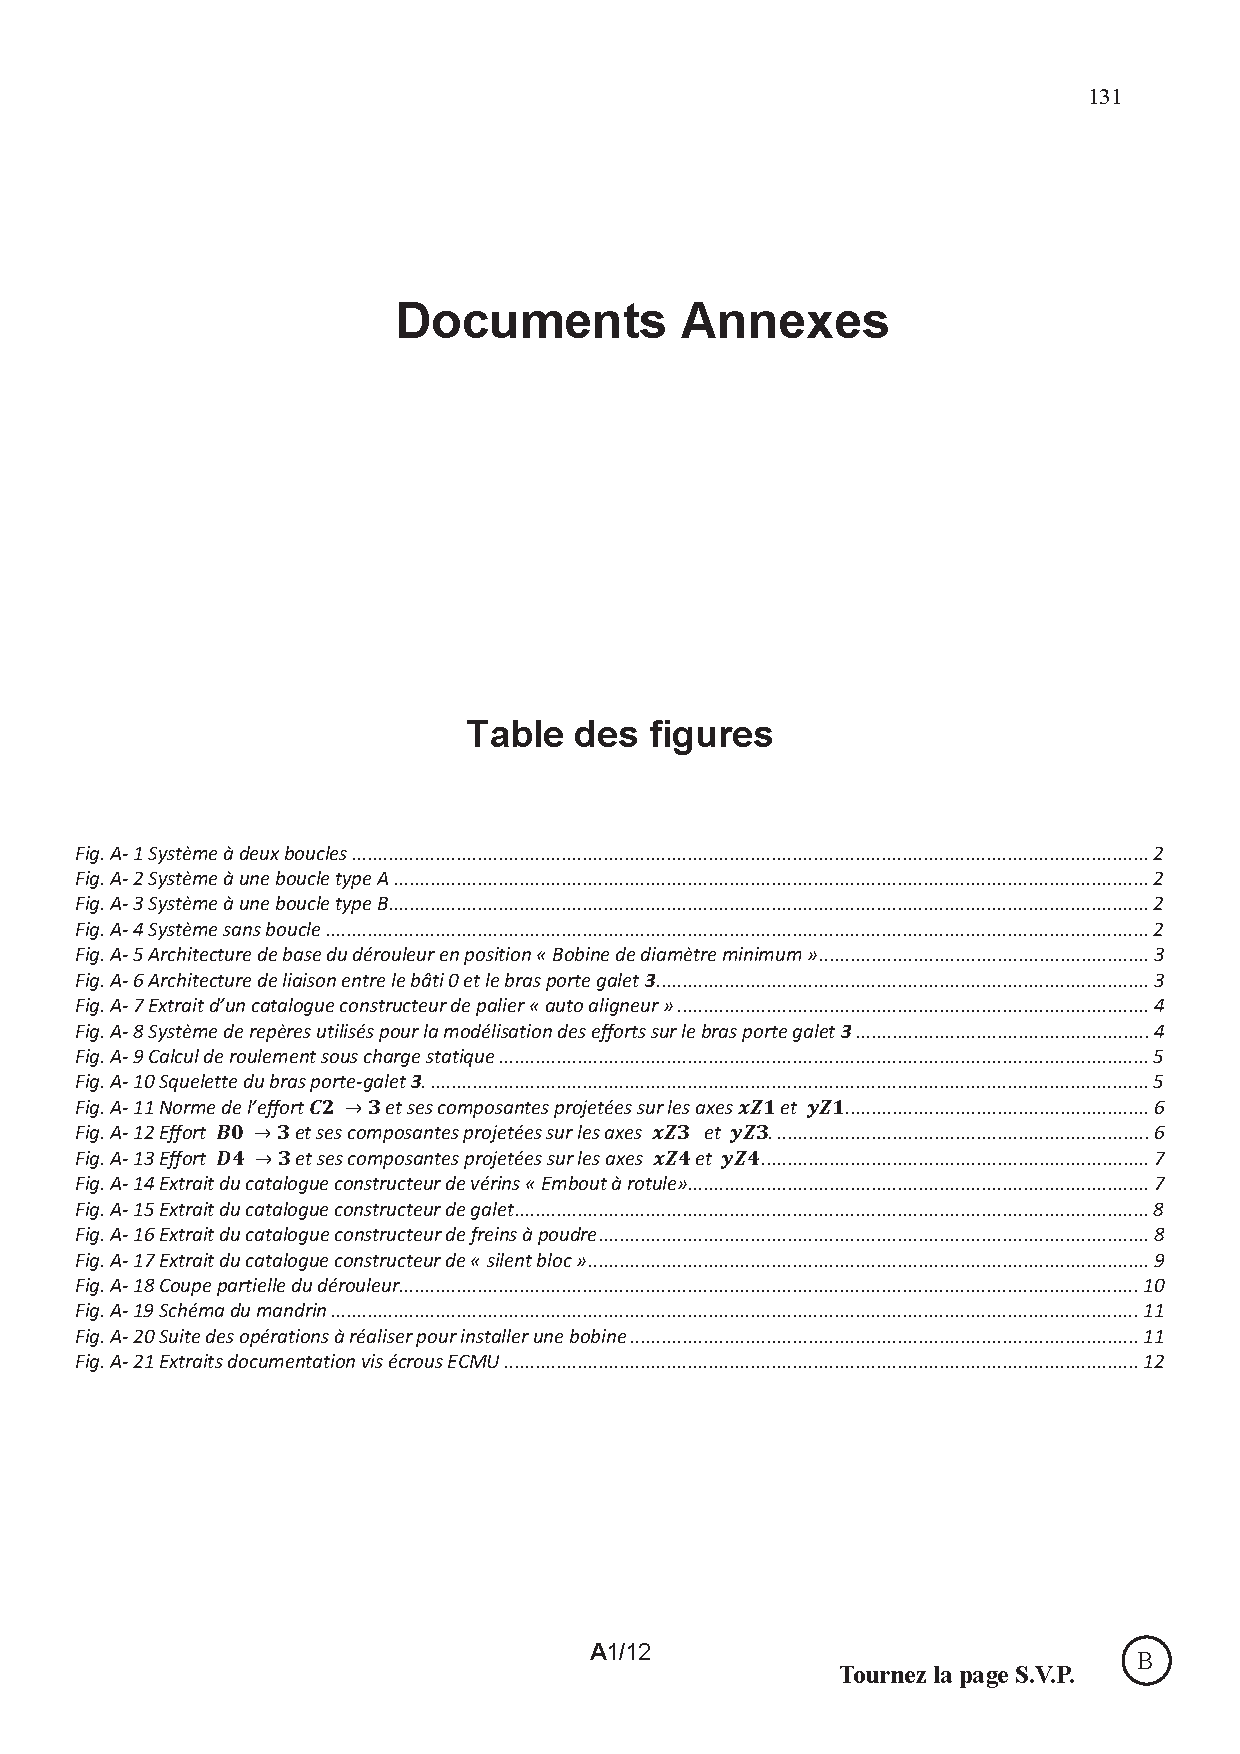
\includepdf[offset=5mm -10mm 0mm 0mm,pages=1]{img/annexes.pdf}

\newpage
\cleardoublepage

\pagestyle{documentreponse}

\section{Document réponse}

\reponse{5}{Efforts normaux et durées des phases de marche pour des marches saine et perturbée.}{Selon la figure 3, en marche saine, les évolutions des efforts normaux sur chaque jambe et les durées de chacune des phases sont identiques. La figure 5 montre que, lors d'une marche perturbée, la phase de double appui est plus longue, 20\% au lieu de 10\% du cycle de marche - phase rassurante et moins douloureuse - et que la jambe invalide (gauche ici) est moins sollicitée avec un temps d'appui plus court (30\% au lieu de 40\%). Les efforts normaux sont en moyenne équivalent en intensité pour les deux marches, cependant leurs évolutions diffèrent dans le cas de la marche perturbée avec un effort quasi constant lors de l'appui de la jambe invalide et un effort également plus constant lors de l'appui de la jambe valide.}

\reponse{5}{Rôle de la canne lors d'une marche assistée.}{La canne prend en charge une partie des efforts normaux supportés par la jambe invalide. En contrepartie, la phase de double appuie s'en trouve encore rallongée.}

\reponse{1}{Transformée de Laplace de l'équation du mouvement et schéma-blocs à compléter.
\begin{center}
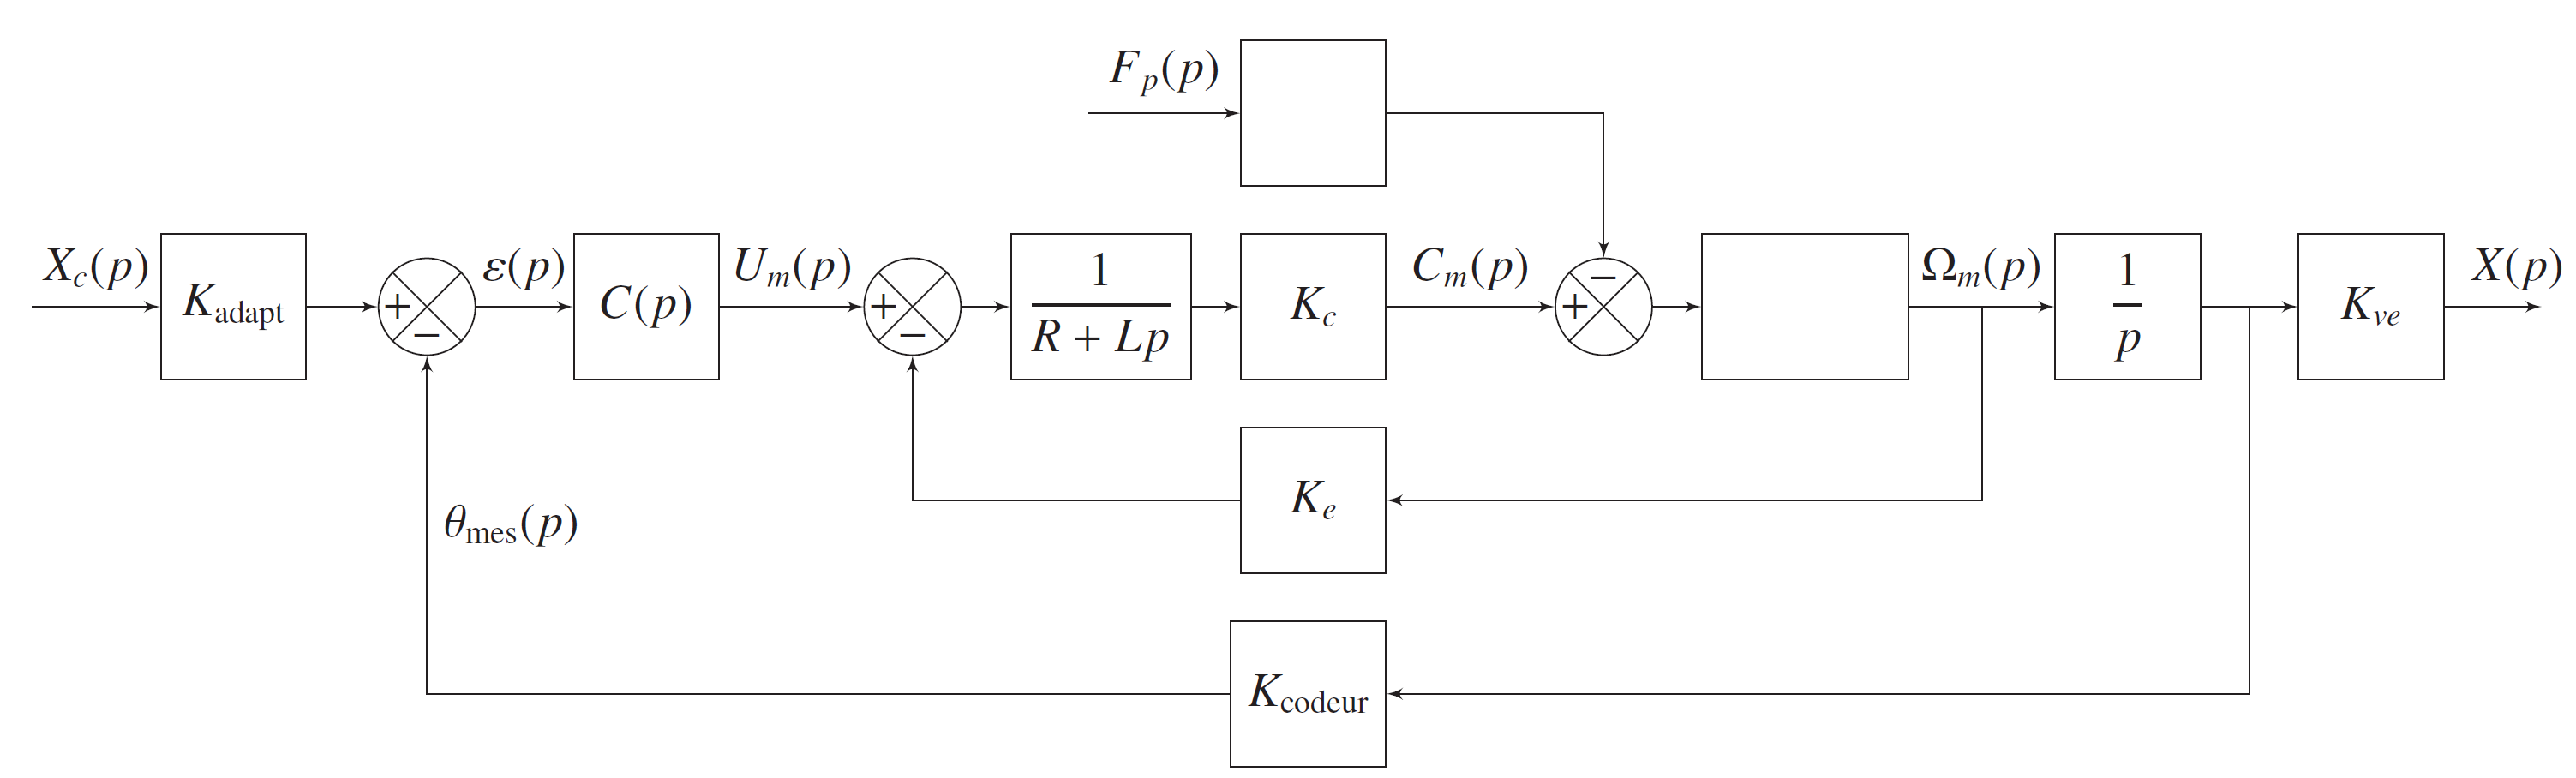
\includegraphics[width=\linewidth]{img/schbloc} 
\end{center}}{$(J_{eq}p+f)\Omega_m(p)=C_m(p)-F_p(p)\dfrac{pas}{2\pi}$
\begin{center}
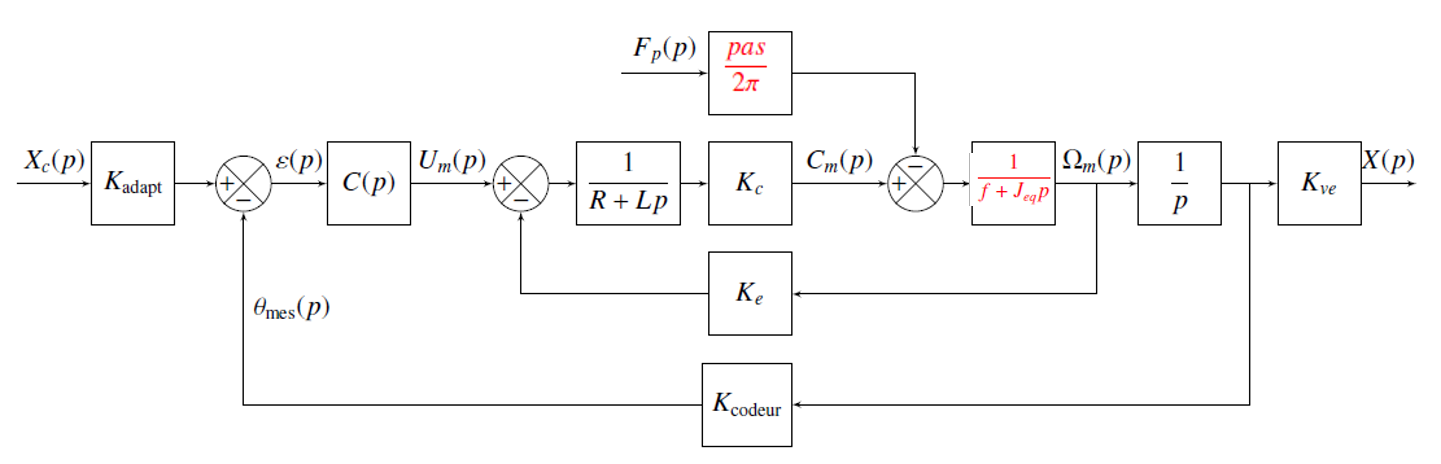
\includegraphics[width=12cm]{img/schbloc_corr} 
\end{center}}

\newpage

\reponse{5}{Expressions littérales sous forme canonique de $H_1(p)$ et $H_2(p)$.}
{$H_1(p)=\dfrac{K_c}{(R+Lp)(J_{eq}p+f)+K_cK_e}=\dfrac{\dfrac{K_c}{Rf+K_cK_e}}{1+\dfrac{RJ+Lf}{Rf+K_cK_e}p+\dfrac{LJ}{Rf+K_cK_e}p^2}$ et

 $H_2(p)=\dfrac{pas}{2\pi}\dfrac{1}{K_c}(R+Lp)H_1(p)=\dfrac{R\dfrac{pas}{2\pi}(1+\dfrac{L}{R}p)}{1+\dfrac{RJ+Lf}{Rf+K_cK_e}p+\dfrac{LJ}{Rf+K_cK_e}p^2}$}

\reponse{2}{Expression de $K_{adapt}$ et application numérique.}
{La condition $\varepsilon=0$ quand $x_c=x$ impose \fbox{$K_{adapt}=\dfrac{K_{codeur}}{K_{ve}}=\dfrac{79,6}{0,477}\approx\dfrac{80}{0,5}\approx\SI{160}{inc /min}$}}

\reponse{2}{Schéma-bloc en fonction de $K_{codeur}$, $K_{ve}$, $C(p)$, $H_1(p)$ et $H_2(p)$. En déduire $H_{BO1}(p)$.
\begin{center}
\begin{tikzpicture}
			\sbEntree{E1}
			\sbComp{C1}{E1}
				\sbRelier[$X_c(p)$]{E1}{C1}
			\sbBloc{B1}{~\hspace{3.5cm}~}{C1}
				\sbRelier{C1}{B1}
			\sbSumh[8]{C2}{B1}
				\sbRelier{B1}{C2}
			\sbBloc[4]{B2}{~\hspace{2.5cm}~}{C2}
				\sbRelier[$\Omega_m(p)$]{C2}{B2}
			\sbSortie[3]{S1}{B2}
				\sbRelier[$X(p)$]{B2}{S1}
			\sbRenvoi{B2-S1}{C1}{}	
			\sbDecaleNoeudy[-4]{C2}{N}
				\sbRelier{N}{C2}
			\sbBloc[-8]{B3}{~\hspace{2cm}~}{N}
				\sbRelierxy{B3}{C2}
			\sbDecaleNoeudx[-7]{B3}{E2}
				\sbRelier[$F_p(p)$]{E2}{B3}
		\end{tikzpicture}
\end{center}}
{\begin{center}
\begin{tikzpicture}
			\sbEntree{E1}
			\sbComp{C1}{E1}
				\sbRelier[$X_c(p)$]{E1}{C1}
			\sbBloc{B1}{$\frac{K_{codeur}}{K_{ve}} C(p) H_1(p)$}{C1}
				\sbRelier{C1}{B1}
			\sbSumh[8]{C2}{B1}
				\sbRelier{B1}{C2}
			\sbBloc[4]{B2}{$\dfrac{K_{ve}}{p}$}{C2}
				\sbRelier[$\Omega_m(p)$]{C2}{B2}
			\sbSortie[3]{S1}{B2}
				\sbRelier[$X(p)$]{B2}{S1}
			\sbRenvoi{B2-S1}{C1}{}	
			\sbDecaleNoeudy[-4]{C2}{N}
				\sbRelier{N}{C2}
			\sbBloc[-8]{B3}{$H_2(p)$}{N}
				\sbRelierxy{B3}{C2}
			\sbDecaleNoeudx[-5]{B3}{E2}
				\sbRelier[$F_p(p)$]{E2}{B3}
		\end{tikzpicture}
\end{center}

$H_{BO1}(p)=K_{codeur} C(p) H_1(p) \dfrac{1}{p}$}


\newpage


\reponse{5}{Tracés asymptotiques de $H_{BO1}(p)$. Valeurs de $T_1$, $T_2$ et $K_{BO}$.

\noindent
\begin{minipage}{.78\linewidth}\centering
\begin{tikzpicture}[xscale=2,]
\begin{scope}[yscale=5/300]
\tikzset{semilog lines/.style={thin, blue},
		 semilog lines2/.style={semilog lines,red!50},
		 semilog half lines/.style={semilog lines 2,dotted},
		 semilog label x/.style={semilog lines,below,font=\tiny},
		 semilog label y/.style={semilog lines,right,font=\tiny}}
\UnitedB
\OrdBode{20}
\semilog{-1}{5}{-200}{20}
\BodeAmp[thick,samples=100,black]{-1:5}{\IntAmp{1}+\POAmp{0.032}{.01}+\POAmp{1}{.0001}}

%\BodeAmp[thick,samples=100]{-2:5}{\IntAmp{1}+\POAmpAsymp{0.032}{.01}+\POAmpAsymp{1}{.0001}}
\end{scope}
\begin{scope}[yshift=-3cm,yscale=5/400]
\tikzset{semilog lines/.style={thin, blue},
		 semilog lines2/.style={semilog lines,red!50},
		 semilog half lines/.style={semilog lines 2,dotted},
		 semilog label x/.style={semilog lines,below,font=\tiny},
		 semilog label y/.style={semilog lines,right,font=\tiny}}
\UniteDegre
\OrdBode{45}
\semilog{-1}{5}{-270}{-90}
\BodeArg[thick,samples=100,black]{-1:5}{\IntArg{1}+\POArg{0.032}{.01}+\POArg{1}{.0001}}
%\BodeArg[thick,samples=100]{-2:5}{\IntArg{1}+\POArgAsymp{0.032}{.01}+\POArgAsymp{1}{.0001}}
\end{scope}
\end{tikzpicture}
\captionof{figure}{Diagrammes de Bode de $H_{BO}$\label{bode0}}
\end{minipage}\hfill
\begin{minipage}{.15\linewidth}
	\feuilleDR{8cm}
\end{minipage}
}{Tracés asymptotiques de $H_{BO1}(p)$. Valeurs de $T_1$, $T_2$ et $K_{BO}$.

\noindent
\begin{minipage}{.78\linewidth}\centering
\begin{tikzpicture}[xscale=2,]
\begin{scope}[yscale=5/300]
\tikzset{semilog lines/.style={thin, blue},
		 semilog lines2/.style={semilog lines,red!50},
		 semilog half lines/.style={semilog lines 2,dotted},
		 semilog label x/.style={semilog lines,below,font=\tiny},
		 semilog label y/.style={semilog lines,right,font=\tiny}}
\UnitedB
\OrdBode{20}
\semilog{-1}{5}{-200}{20}
\BodeAmp[thick,samples=100,black]{-1:5}{\IntAmp{1}+\POAmp{0.032}{.01}+\POAmp{1}{.0001}}
\BodeAmp[thick,samples=100]{-2:5}{\IntAmp{1}+\POAmpAsymp{0.032}{.01}+\POAmpAsymp{1}{.0001}}
\end{scope}
\begin{scope}[yshift=-3cm,yscale=5/400]
\tikzset{semilog lines/.style={thin, blue},
		 semilog lines2/.style={semilog lines,red!50},
		 semilog half lines/.style={semilog lines 2,dotted},
		 semilog label x/.style={semilog lines,below,font=\tiny},
		 semilog label y/.style={semilog lines,right,font=\tiny}}
\UniteDegre
\OrdBode{45}
\semilog{-1}{5}{-270}{-90}
\BodeArg[thick,samples=100,black]{-1:5}{\IntArg{1}+\POArg{0.032}{.01}+\POArg{1}{.0001}}
\BodeArg[thick,samples=100]{-2:5}{\IntArg{1}+\POArgAsymp{0.032}{.01}+\POArgAsymp{1}{.0001}}
\end{scope}
\end{tikzpicture}
\captionof{figure}{Diagrammes de Bode de $H_{BO}$\label{bode0}}
\end{minipage}\hfill
\begin{minipage}{.15\linewidth}
	\feuilleDR{8cm}
\end{minipage}

On obtient $\omega_{c1}=10^4 \SI{}{rad/s}$ donc $ T_1 = 10^{-4}s=\SI{0.1}{ms}$, et $\omega_{c2}=10^2 \SI{}{rad/s}$ donc $ T_2 = 10^{-2}s=\SI{10}{ms}$.

On a aussi $20\log(K_{BO}) = \SI{-30}{dB}$ d'où $K_{BO}=10^{\frac{-30}{20}}=\SI{0.032}{}$.}

\reponse{2}{Justification de la modélisation approchée.}
{$F_{MAX} =\SI{4}{Hz}$ correspond à une sollicitation de pulsation $\omega_{MAX} = 4\times2\pi=\SI{25}{rad/s}$.
On constate que $\omega_{MAX} < \omega_{c2} = \SI{100}{rad/s} \ll \omega_{c1} = 10^4 rad/s$.
Pour $\omega < \omega_{MAX}$, le système se comporte donc comme un intégrateur pur de gain égal à $K_{BO}$. L'approximation de $H_{BO}(p)$ par $\dfrac{K_{BO}}{p}$ avec $K_{BO}= \dfrac{1}{30} \approx 0.032 $ est donc acceptable.}

\reponse{2.5}{Expression littérale sous forme canonique de $H_{BF}(p)$}
{$H_{BF}(p) = \dfrac{X(p)}{Xc(p)} = \dfrac{K_{corr}\dfrac{K_{BO}}{p}}{1+K_{corr}\dfrac{K_{BO}}{p}}=\dfrac{1}{1+\dfrac{1}{K_{corr}K_{BO}}p}$}

\reponse{4}{Paramètres de $H_{BF}(p)$ et performances pour $K_{corr} = 1$. Conclusions vis-à-vis des exigences.}{Avec $K_{corr} = 1$, $H_{BF}(p) =\dfrac{1}{1+\frac{p}{K_{BO}}}$, donc 1er ordre, $K=1$ et $\tau=\frac{1}{K_{BO}}$.

On en déduit que la gain est unitaire et que la constante de temps est $\tau = \dfrac{1}{K_{BO}}=\SI{30}{s}$.

Les performances de ce système sont donc :
\begin{itemize}
\item système stable car système du 1er ordre $\rightarrow$ cdc vérifié,
\item système précis car de gain unitaire $\rightarrow$ cdc vérifié,
\item système ne présente pas de dépassement car système du 1er ordre $\rightarrow$ cdc vérifié,
\item $tr_{5\%} = 3 \times 30 = \SI{90}{s} \rightarrow$ cdc non vérifié car le temps de réponse attendu est de \SI{60}{ms}.
Le système avec $K_{corr} = 1$ est donc trop lent.
\end{itemize}}

\reponse{3}{Influence du gain $K_{corr}$ sur les diagrammes de Bode.}
{L'augmentation du gain $K_{corr}$ entraîne une translation de la courbe de gain uniquement selon l'axe des ordonnées.}

\reponse{3}{Valeur de $K_{corr}$ pour assurer l'exigence de rapidité.}{Il faut augmenter $K_{corr}$, tel que $tr_{5\%} = 3 \times \frac{1}{K_{corr}.K_{BO}} \le 60$ ms. Donc \\
$K_{corr} \ge \dfrac{3}{60.10^{-3}.K_{BO}}$.
L'application numérique donne $K_{corr} \ge  1500$.}

\reponse{3}{Le modèle est-il cohérent? Justifier. Quel(s) changement(s) faudrait-il faire ?}{L'allure de la réponse ne correspond pas à celle d'un système du $1^{er}$ ordre car un dépassement est observé. Avec $K_{corr} = 1500$, le système en boucle ouverte ne peut plus être modélisé par un intégrateur pur de gain $K_{BO}$, en effet cette valeur élevée de $K_{corr}$ fait monter la courbe de gain, le système a une bande passante plus élevée et l'action du terme $\frac{1}{1+T_2.p}$ ne peut plus être négligée. Le comportement du système doit donc être modélisé par celui d'un système du second ordre pour se rapprocher du comportement observé.}

\newpage

\reponse{4.5}{Donner la nouvelle $H_{BF}(p)$ et identifier ses paramètres caractéristiques.}
{$H_{BF}(p)=\dfrac{K_{corr}\dfrac{K_{BO}}{p(1+\tau_{BO}p)}}{1+K_{corr}\dfrac{K_{BO}}{p(1+\tau_{BO}p)}}=\dfrac{1}{1+\dfrac{1}{K_{corr}K_{BO}}p+\dfrac{\tau_{BO}}{K_{corr}K_{BO}}p^2}$

D'où le gain est unitaire, $\omega_0=\sqrt{\dfrac{K_{corr}K_{BO}}{\tau_{BO}}}$ et $z=\dfrac{1}{2\sqrt{\tau_{BO}K_{corr}K_{BO}}}$}

\reponse{3}{Valeur de $K_{corr}$ qui permet de vérifier les critères de précision et de dépassement.}{Le critère de précision est satisfait car gain unitaire.\\
Pour assurer un 1er dépassement $D1\% \leq 5 \%$, il faut que le système du second ordre ait un coefficient d'amortissement $z$, tel que $z \ge 0,7$ donc $K_{corr} \leq \frac{1}{(2 \times 0,7)^2.\tau_{BO}.K_{BO}}$.\\
L'application numérique donne $K_{corr} \leq 1700$. On prend donc $K_{corr}^{MAX} = 1700$.}

\reponse{3}{Valeur de $tr_{5\%}$ de ce modèle pour $K_{corr}=K_{corr}^{MAX}$}{D'après l'abaque du temps de réponse réduit, pour $z = 0,7$ on relève $tr_{5\%}.\omega_0 \simeq 3$. Or $\omega_0 = \sqrt{\frac{K_{corr}^{MAX}.K_{BO}}{\tau_{BO}}} $, donc $tr_{5\%} = 3.\sqrt{\frac{\tau_{BO}}{K_{corr}^{MAX}.K_{BO}}}$. \\
L'application numérique donne : $tr_{5\%} \simeq $ 38 ms $<$ 60 ms $ \Rightarrow $ cdc vérifié !}

\reponse{3}{Conclusion sur le correcteur proportionnel vis-à-vis des exigences.}{Les performances de stabilité, rapidité et de 1er dépassement sont vérifiées. Cependant, le système avec correction proportionnelle n'arrive pas à atténuer suffisamment la perturbation (l'erreur est de l'ordre de 15 à 20$\%$ bien supérieure au 5$\%$ du cahier des charges). Un autre type de correction doit donc être envisagé pour satisfaire l'ensemble des critères.}

\newpage

\reponse{2}{Nouvelle expression de $FTBO(p)$.}{$FTBO(p)=C(p).H_{BO}(p)$, on retrouve l'expression demandée.}

\reponse{2}{Justification et détermination de $\omega_1$ et $\omega_2$.}{Si $\omega<\frac{1}{a}$, alors $1+ja\omega$, alors $a\omega<1$, donc on peut négliger $ja\omega$ devant $1$. Ainsi, $\omega_1=\frac{1}{0,2}=\SI{5}{rad/s}$ et $\omega_2=\frac{1}{9.10^{-3}}=\SI{111}{rad/s}$.}

\reponse{3}{
\begin{center}
\begin{tabular}{|c|c|c|c|}
\hline
$\omega$ & $-\infty$ \hfill $\omega_1$ & $\omega_1$ \hfill $\omega_2$ & $\omega_2$ \hfill $+\infty$ \\ \hline
~\  & ~\ & ~\  & ~\ \\ 
~\  & ~\ & ~\  & ~\ \\ 
~\  & ~\ & ~\  & ~\ \\ 
~\  & ~\ & ~\  & ~\ \\ \hline
Phase & ~\ & ~\ & ~\ \\ \hline
Pente & ~\ & ~\ & ~\ \\
\hline
\end{tabular}
\end{center}
}{
\begin{center}
\begin{tabular}{|c|c|c|c|}
\hline
$\omega$ & $-\infty$ \hfill $\omega_1$ & $\omega_1$ \hfill $\omega_2$ & $\omega_2$ \hfill $+\infty$ \\ \hline
~\  & ~\ & ~\  & ~\ \\ 
$FTBO(p)$ & $\dfrac{K_{BO}.K_{corr}}{p^2}$ & $\dfrac{K_{BO}.K_{corr}.T_d}{p}$ & $\dfrac{K_{BO}.K_{corr}}{p^2}$ \\
~\  & ~\ & ~\  & ~\ \\ \hline
Phase & -180 & -90 & -180 \\ \hline
Pente & -40dB/decade & -20dB/decade & -40dB/decade\\
\hline
\end{tabular}
\end{center}
}

\reponse{2}{Justifier le comportement asymptotique.}{Les résultats trouvés précédemment correspondent aux tracés asymptotiques de la figure.}

\newpage

\reponse{2}{Mise en place du saturateur sur le schéma-bloc.}{Le saturateur en courant doit être placé entre le bloc $\dfrac{1}{R+L.p}$ et le bloc $K_c$.}

\reponse{2}{Influence de la présence du saturateur. Conclusions sur les exigences du cahier des charges.}{Cela diminue sensiblement les oscillations donc, cela améliore la réponse du système.}

\reponse{3}{Première fermeture géométrique.}{On peut écrire la fermeture géométrique suivante : $\vv{IA} + \vv{AH} = \vv{IH} $, c'est à dire $R.\vv{y}_0 + \ell(t).\vv{y}_2=x.\vv{x}_0+h.\vv{y}_0 $.\\
Par projection sur $\vv{y}_0$, il vient :
\begin{center}
$R + \ell(t).cos(\theta(t)) = h= h_0 $
\end{center}
}

\reponse{3}{Deuxième fermeture géométrique.}{La fermeture géométrique $\vv{IA} + \vv{AH} = \vv{IH}$ s'écrit avec le paramétrage donné :\\
$R.\vv{j}_0 + \ell.\vv{j}_3 = \lambda(t).\vv{v}$. En projetant cette équation dans la base $\mathcal{R}_0$, on obtient :\\
$/\vv{i}_0 : 0 - \ell.sin(\theta) = - \lambda.sin(\beta)$ (eq1)\\
$/\vv{j}_0 : R + \ell.cos(\theta) = \lambda.cos(\beta)$ (eq2)\\
On obtient la relation demandée en éliminant le paramètre $\lambda$. Pour cela on considère $\frac{(eq1)}{(eq2)}$ en s'assurant que $\beta \neq \pi/2$, il vient :\\
$tan(\beta) = \frac{\ell.sin(\theta)}{R + \ell.cos(\theta)}$
}

\reponse{3}{Équation reliant $\beta$ et $\theta$.}{
$tan(\beta) = \frac{\ell.sin(\theta)}{R + \ell.cos(\theta)}= \frac{\ell.sin(\theta)}{h}= \frac{\ell.sin(\theta)}{h}\cdot\frac{h-R}{\ell\cdot\cos(\theta)}= \frac{h-R}{h}\cdot\tan(\theta)$
}

\newpage

\reponse{0}{Compléter les vues manquantes.
\begin{figure}[!h]\centering
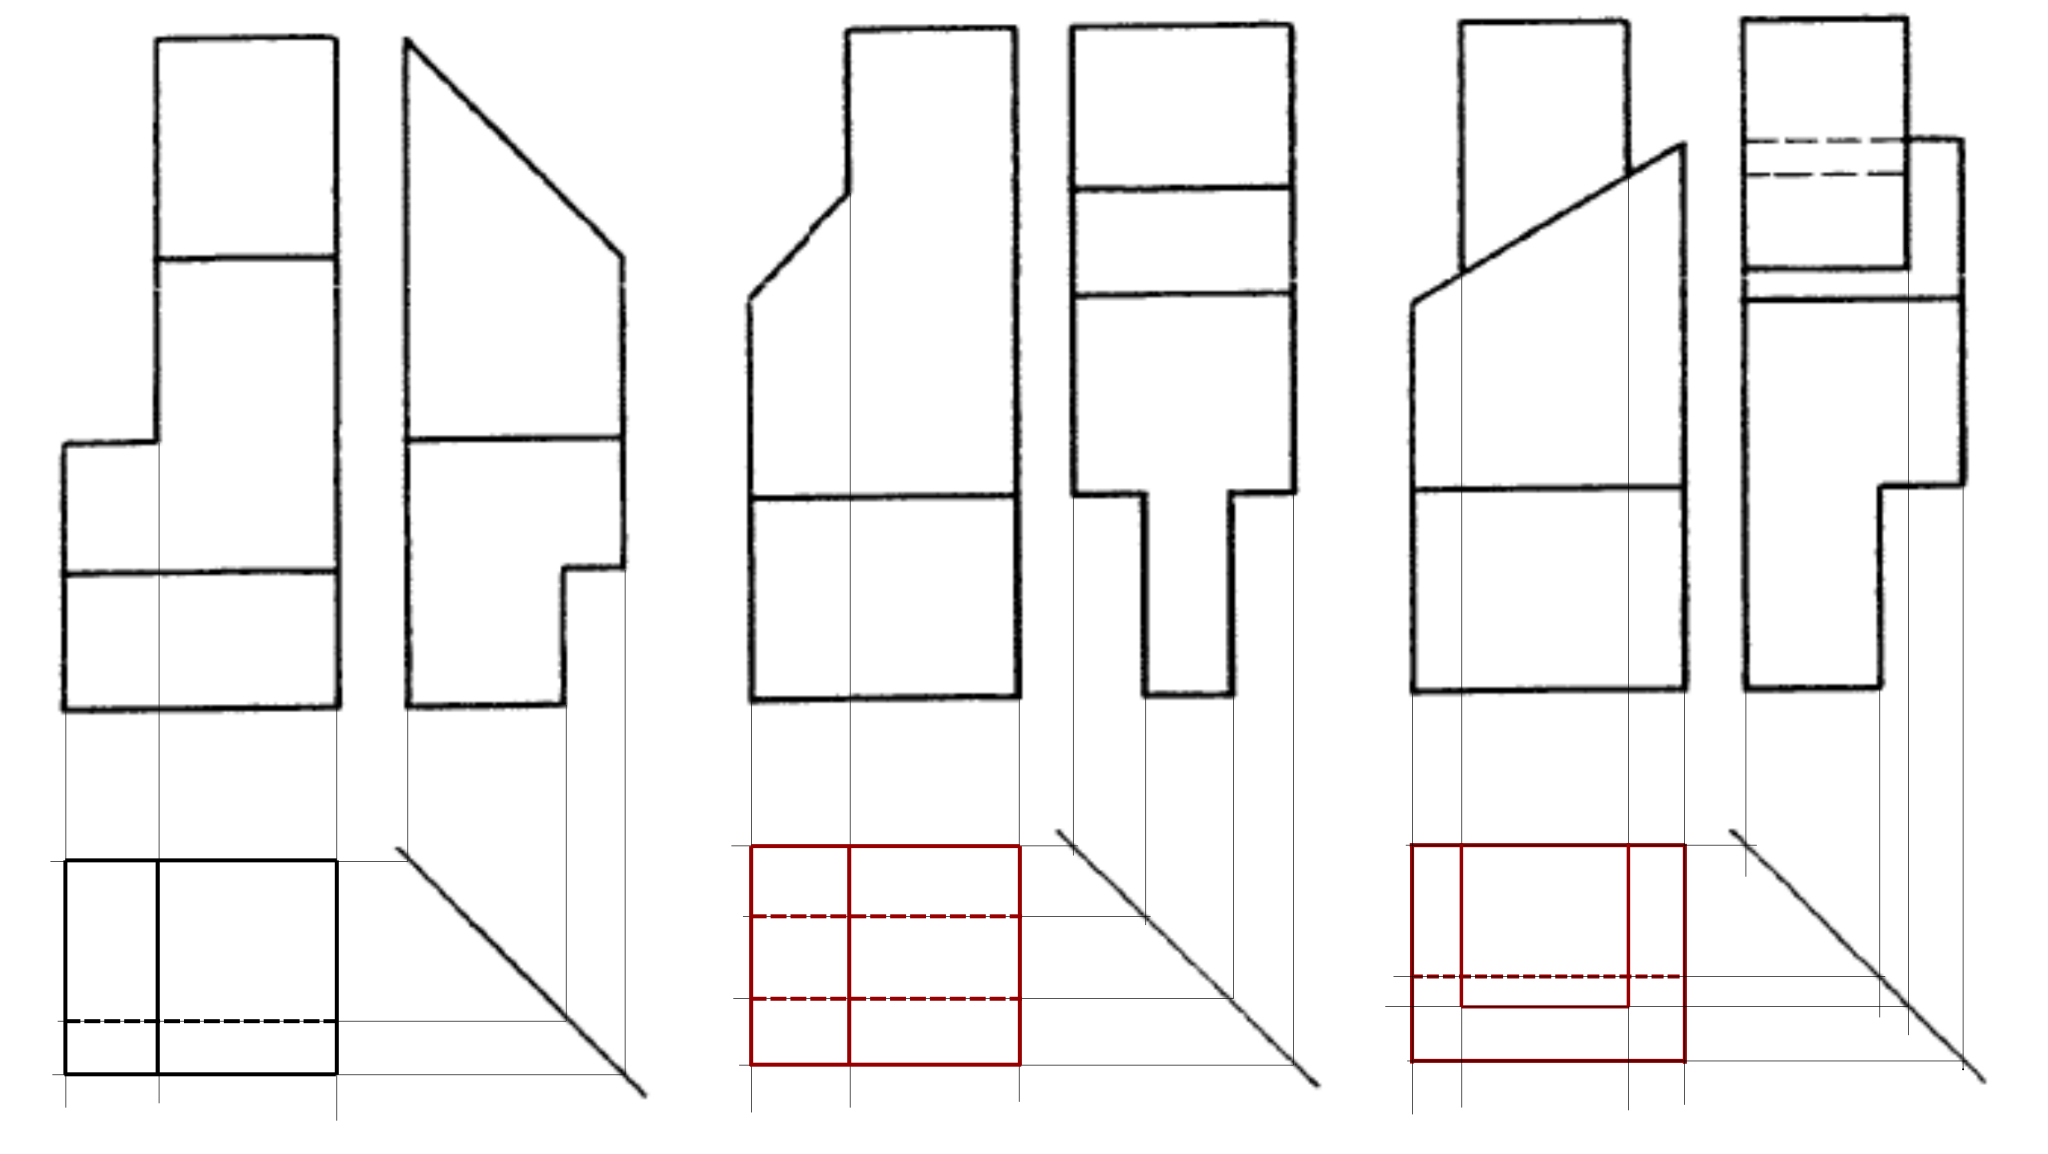
\includegraphics[width=\linewidth]{img/vues_a_completer1}
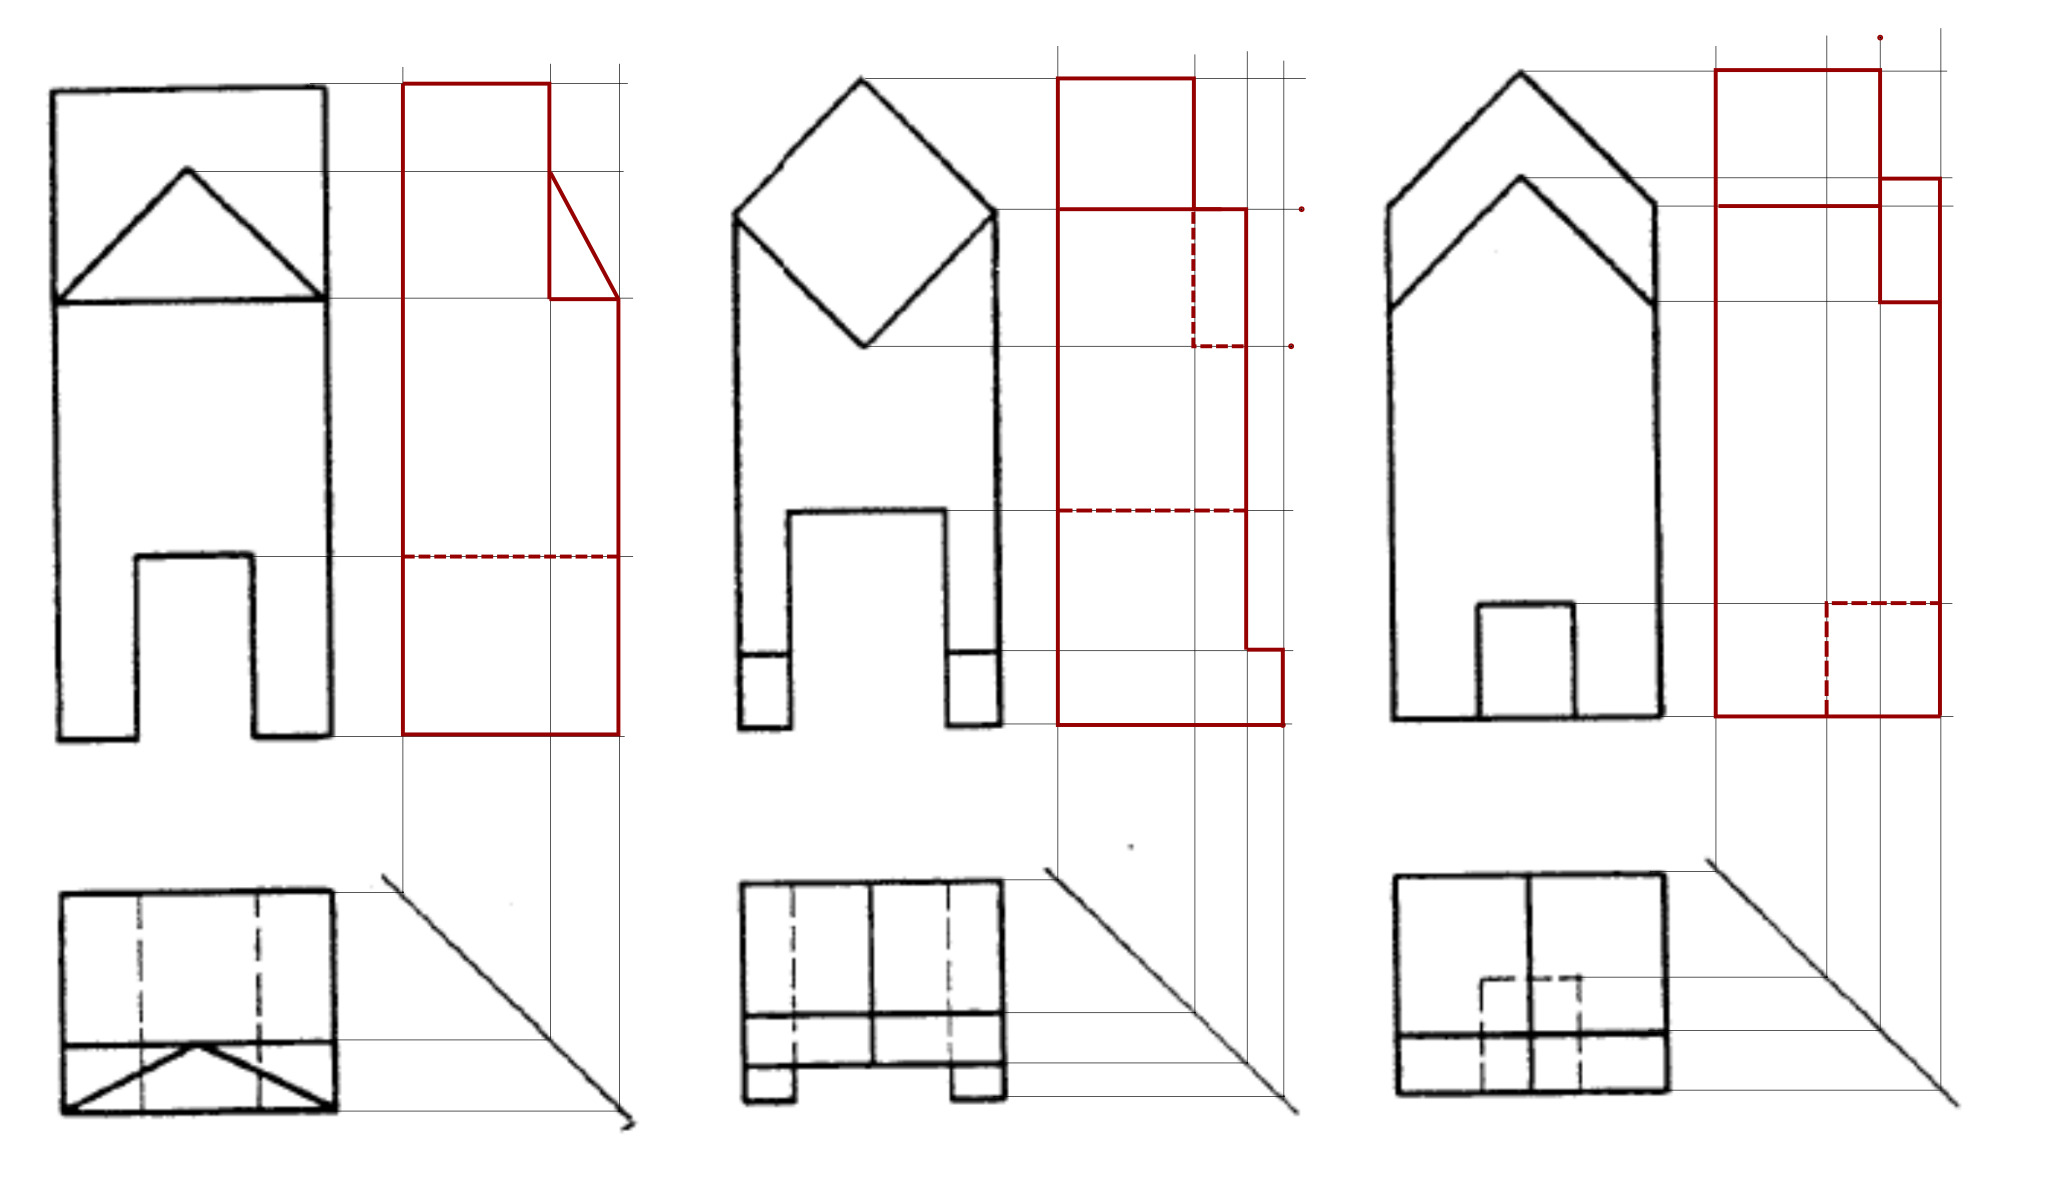
\includegraphics[width=\linewidth]{img/vues_a_completer2}
\caption{\label{vues_a_completer}Vues à compléter}
\end{figure}
}{
\begin{figure}[!h]\centering
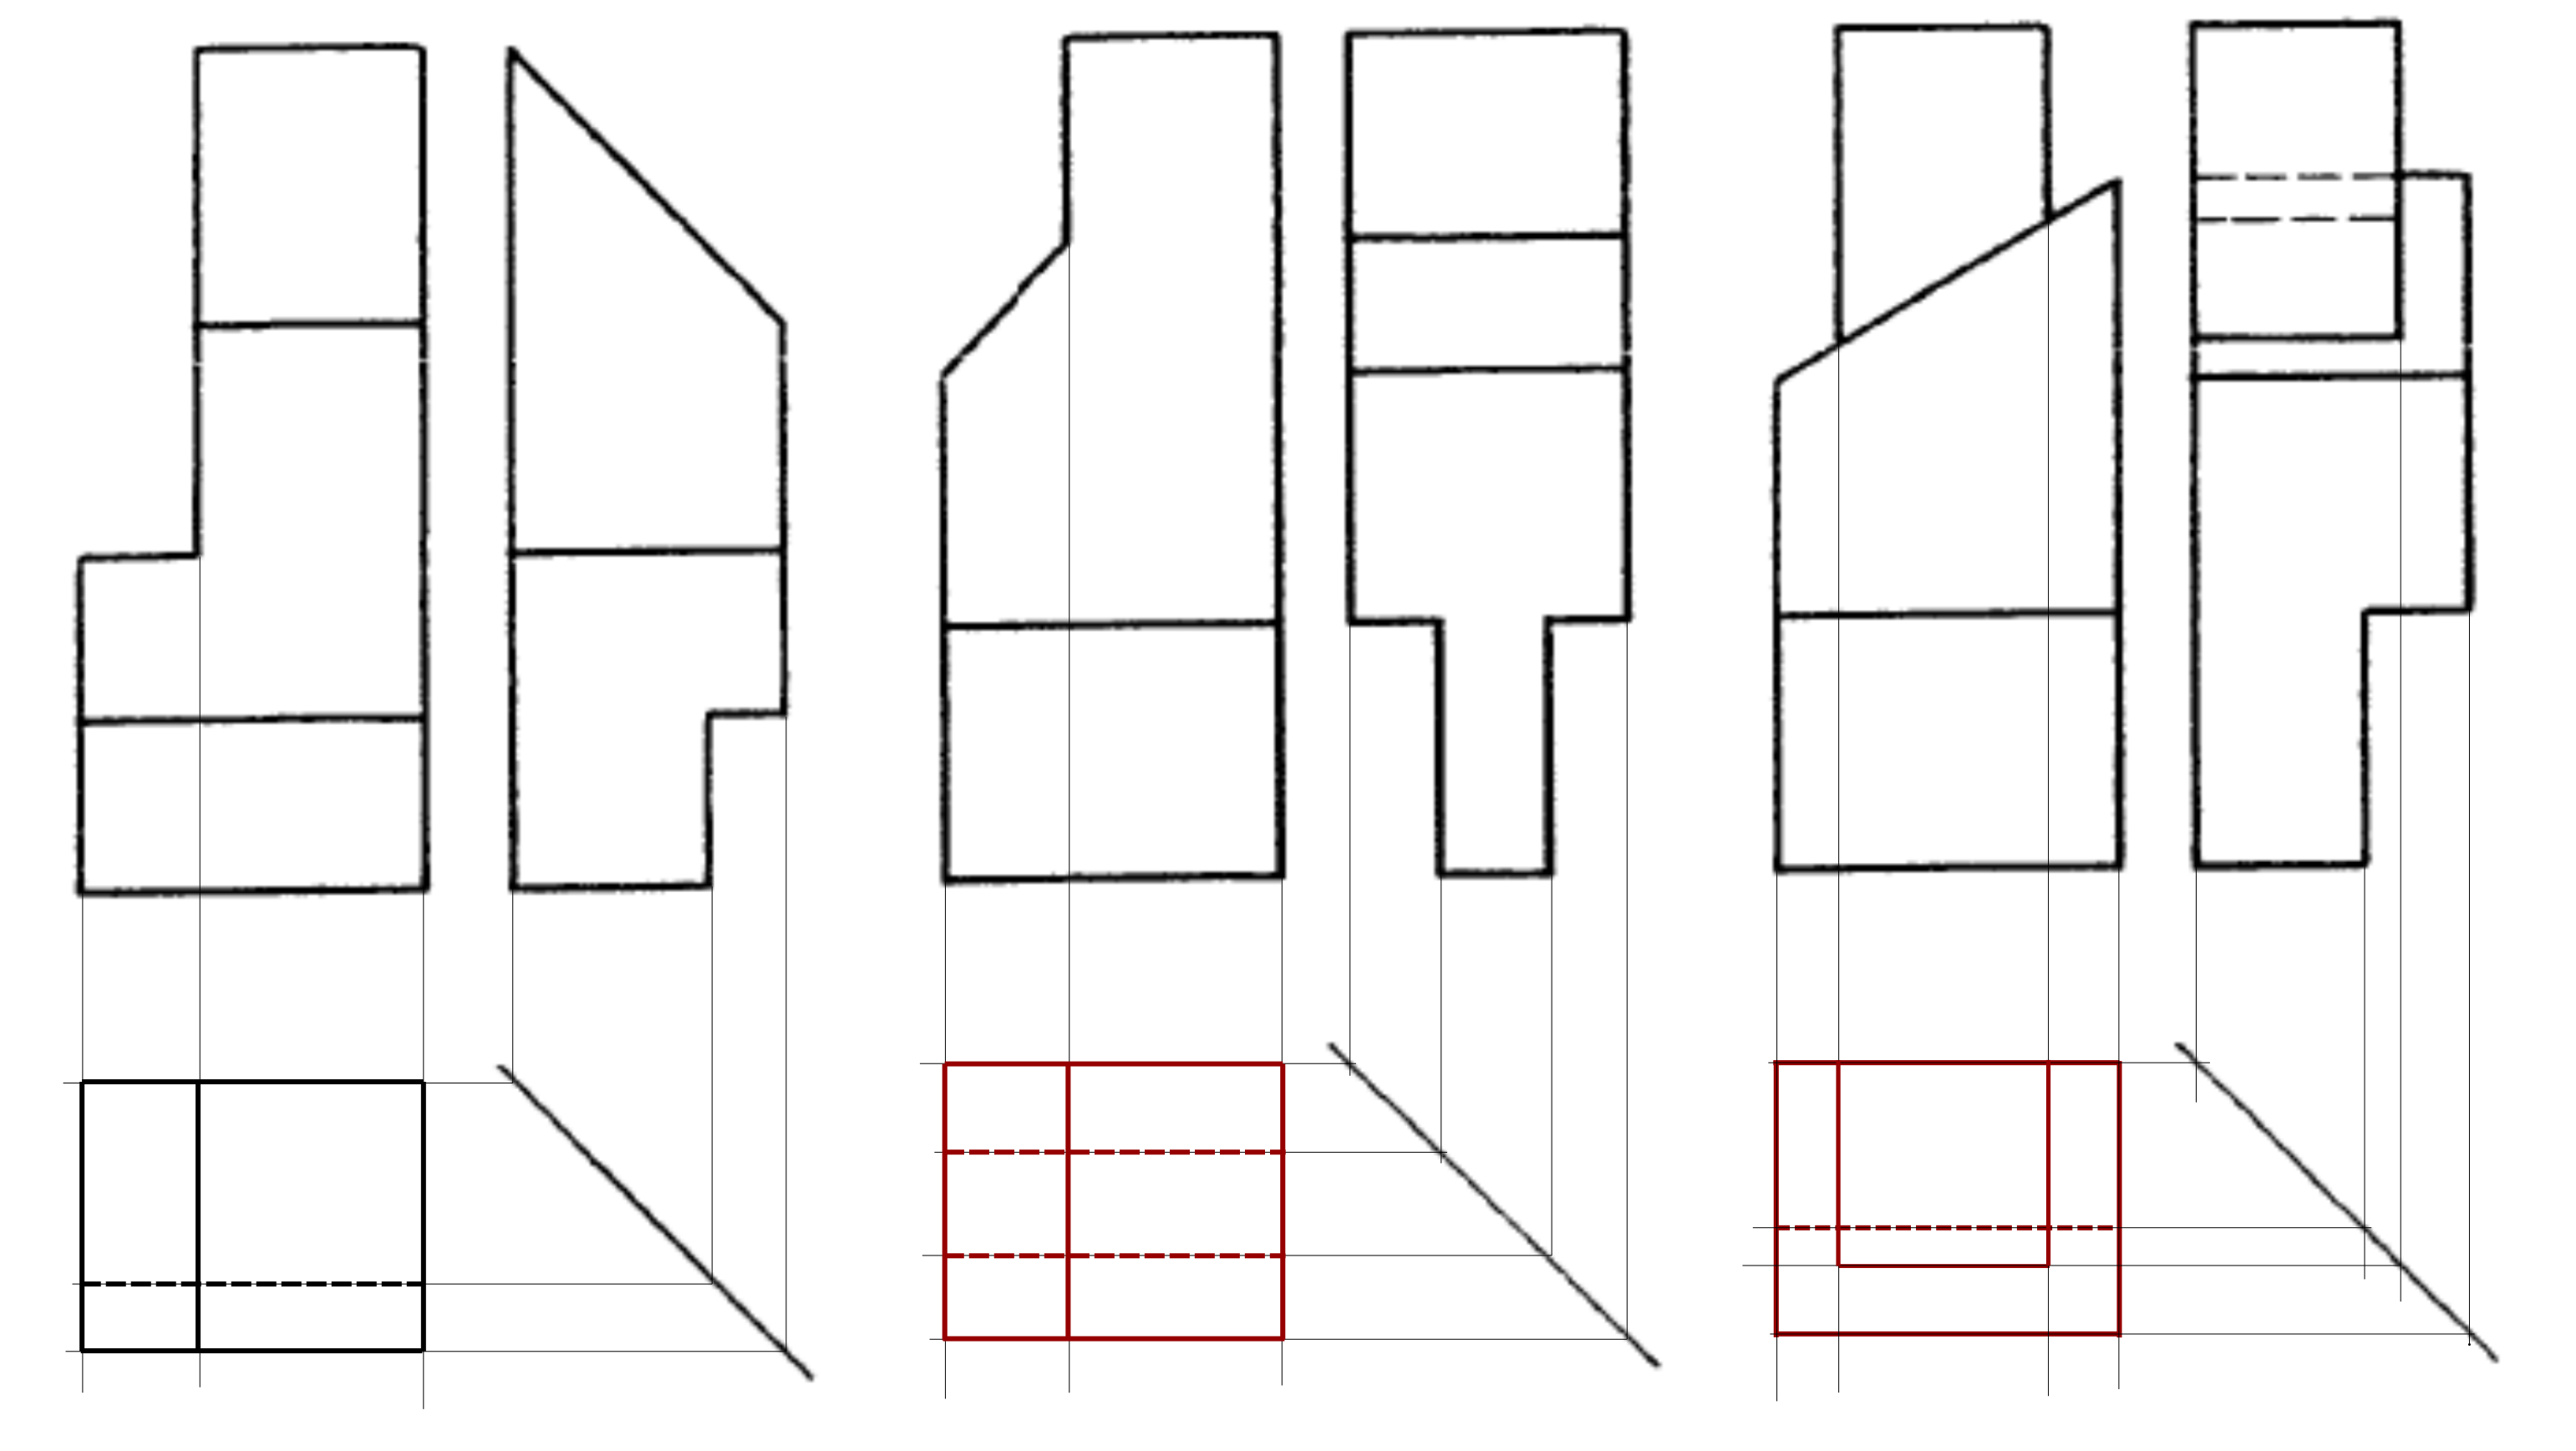
\includegraphics[width=\linewidth]{img/vues_a_completer1_cor}
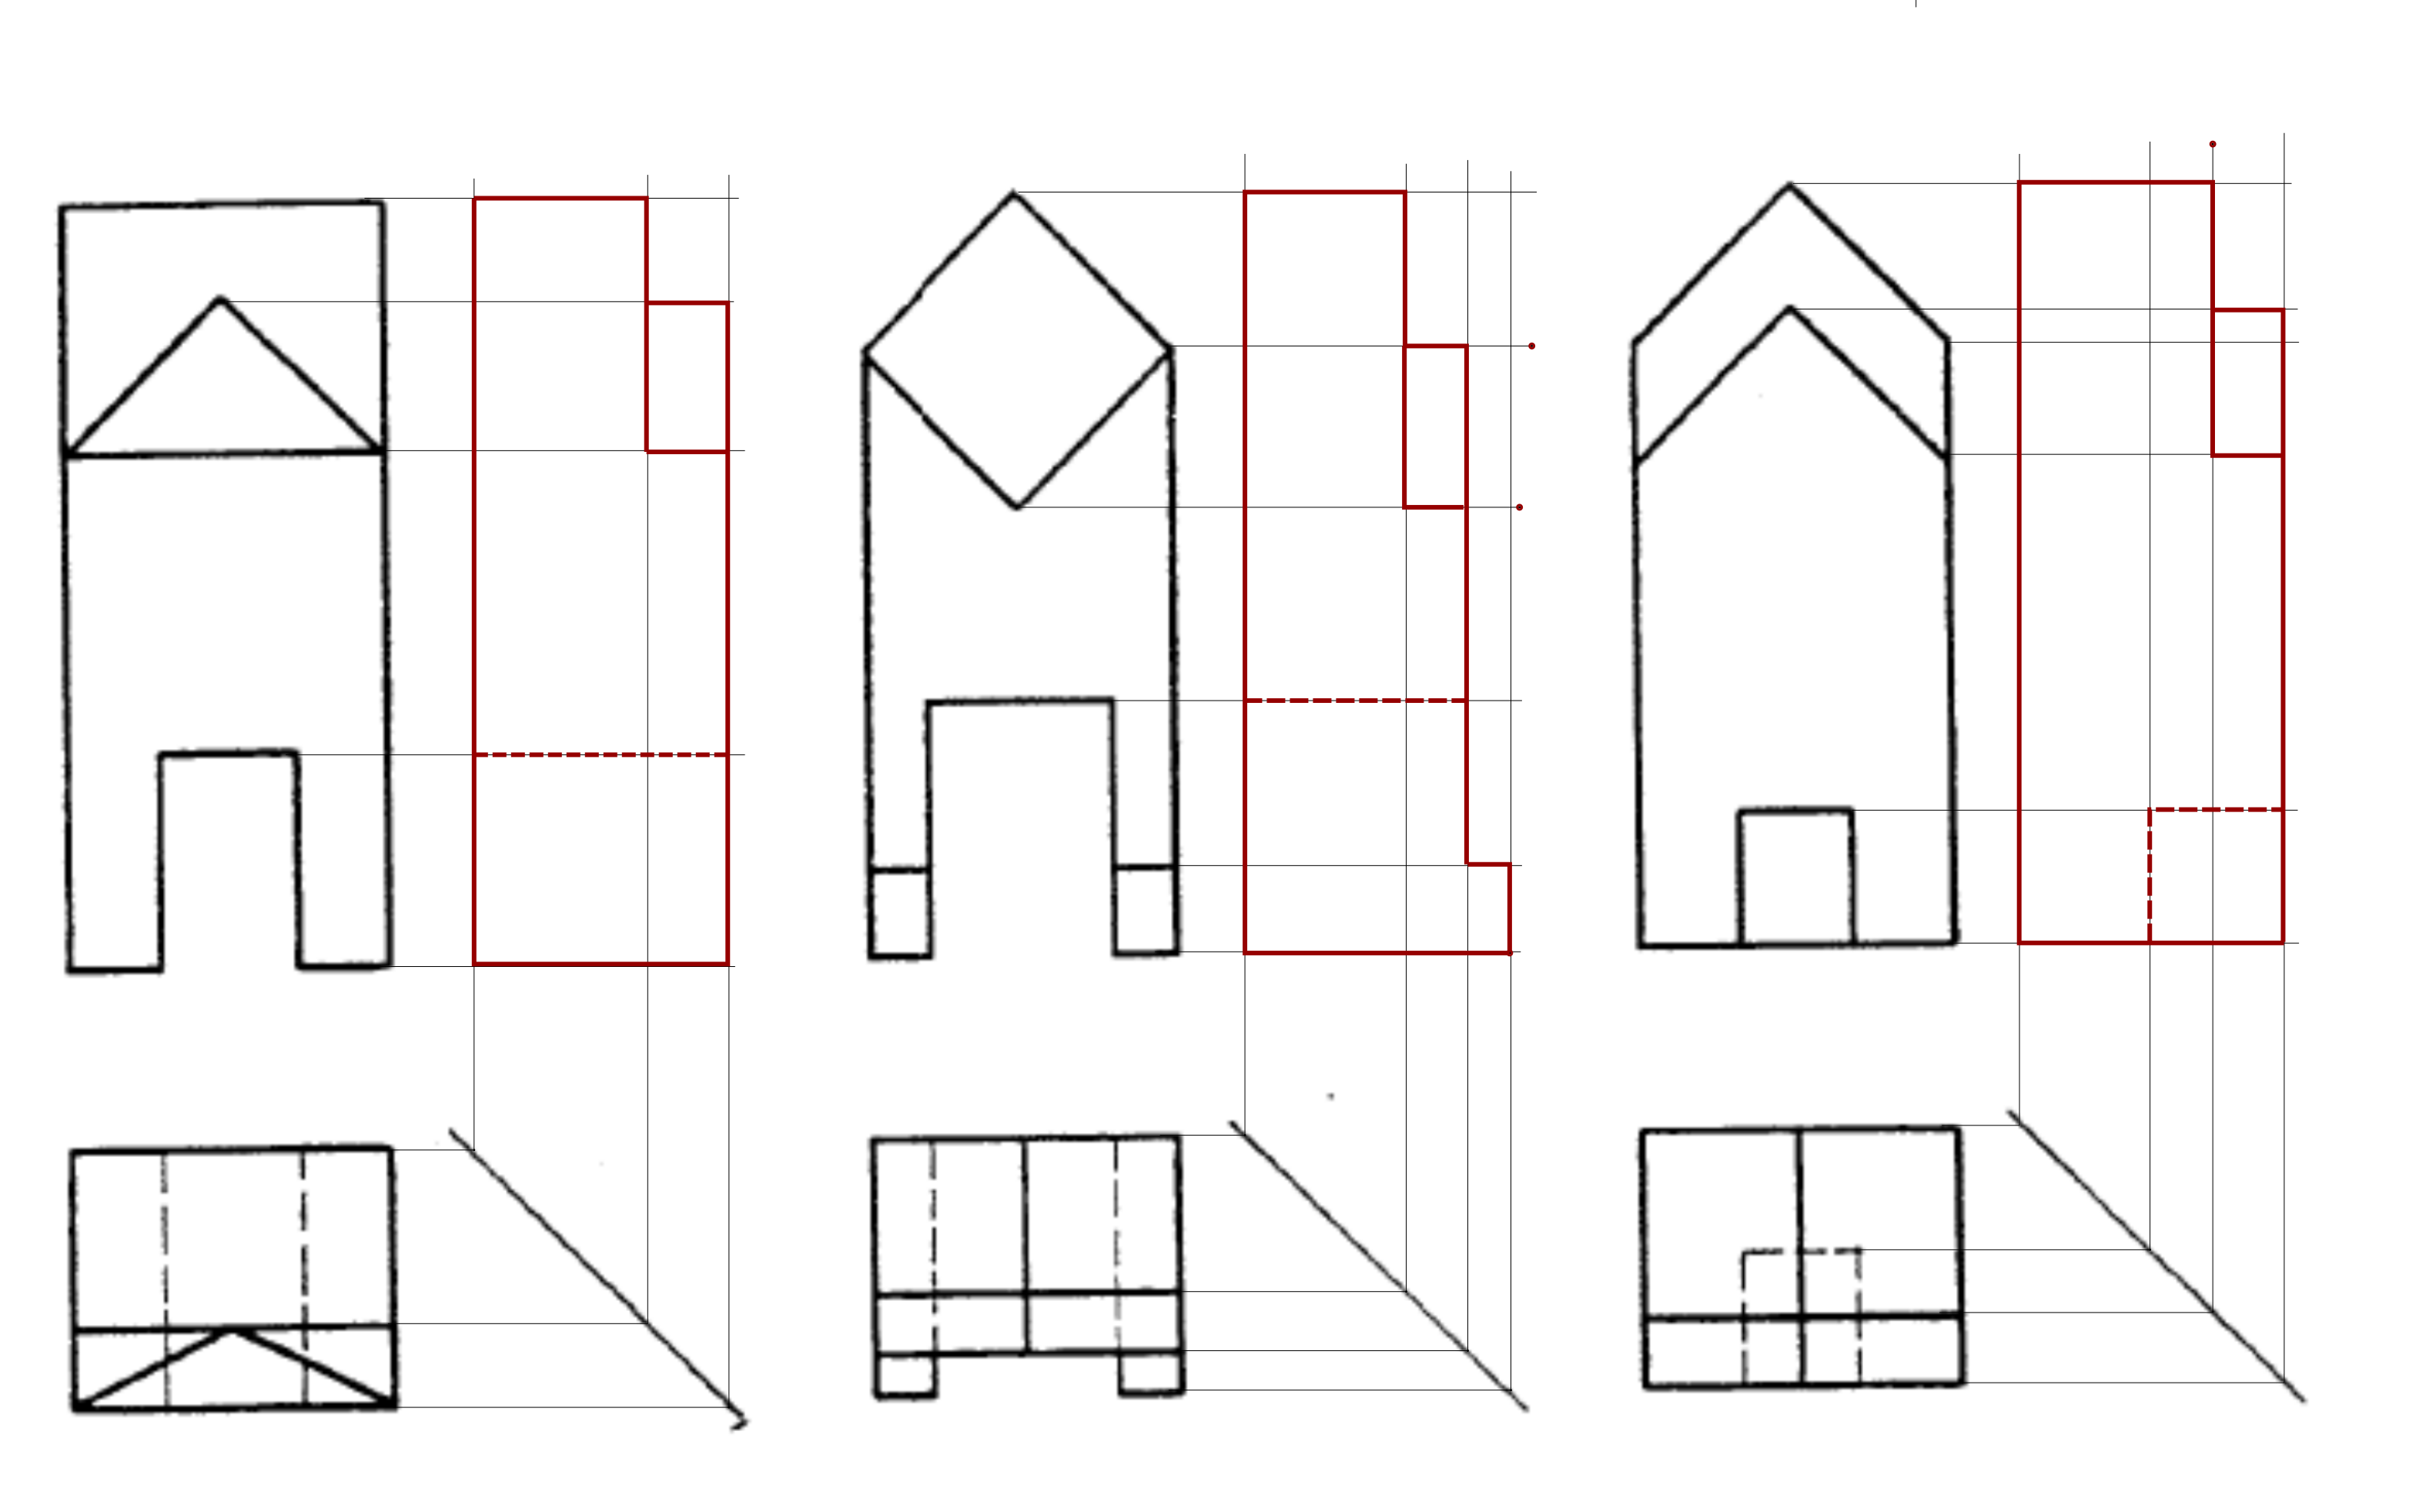
\includegraphics[width=\linewidth]{img/vues_a_completer2_cor}
\caption{\label{vues_a_completer}Vues à compléter}
\end{figure}
}


\end{document}
